\documentclass[aspectratio=169]{beamer}
\usepackage[english]{babel}				% Set language
\usepackage[utf8]{inputenc}			% Set encoding
\usepackage{tikz}
\usepackage{svg}

\usepackage{ifthen}

\usetikzlibrary{calc}

\mode<presentation>						% Set options
{
  \usetheme{default}					% Set theme
  \usecolortheme{default} 				% Set colors
  \usefonttheme{default}  				% Set font theme
  \setbeamertemplate{caption}[numbered]	% Set caption to be numbered
}


% emojis
\usepackage{fontawesome}
%\usepackage{fontspec}
%\newfontfamily\DejaSans{DejaVu Sans}

%\usecolortheme[named=UBCblue]{structure}
\setbeamercolor{math text}{fg=black!30!blue}

% Uncomment this to have the outline at the beginning of each section highlighted.
%\AtBeginSection[]
%{
%  \begin{frame}{Outline}
%    \tableofcontents[currentsection]
%  \end{frame}
%}

\usepackage{graphicx}					% For including figures
\usepackage{booktabs}					% For table rules
\usepackage{hyperref}					% For cross-referencing
\usepackage[backend=biber]{biblatex}
\usepackage{csquotes}
\usepackage{bookmark}
\usepackage{colortbl}                   % For color line
\usepackage{framed}                     % For frames

\beamertemplatenavigationsymbolsempty
\setbeamertemplate{footline}[frame number]

\setbeamerfont{author}{size=\large}
\setbeamerfont{date}{size=\scriptsize}
\setbeamercolor{date}{fg=gray}
\defbeamertemplate*{title page}{customized}[1][]
{
  \centering
  \vspace{1cm}
  \usebeamerfont{title}\textbf{\inserttitle}\par
  \bigskip
  \usebeamerfont{author}\insertauthor\par
  \medskip
  \usebeamercolor[fg]{date}\usebeamerfont{date}\insertdate\par
}


\definecolor{myred}{RGB}{176, 38, 0}
\definecolor{myorange}{RGB}{255, 170, 0}
\definecolor{myblue}{RGB}{0, 157, 196}
\definecolor{mygreen}{RGB}{0, 140, 65}
\newcommand{\bred}[1]{\textcolor{myred}{\textbf{#1}}}
\newcommand{\borange}[1]{\textcolor{myorange}{\textbf{#1}}}
\newcommand{\bblue}[1]{\textcolor{myblue}{\textbf{#1}}}
\newcommand{\bgreen}[1]{\textcolor{mygreen}{\textbf{#1}}}
\newcommand{\btheme}[1]{\textcolor{black!30!blue}{\textbf{#1}}}
\newcommand{\ntheme}[1]{\textcolor{black!30!blue}{{#1}}}

\newcommand{\mytitle}[1]{\centering{\Huge #1}}

\setbeamercolor{block body alerted}{bg=alerted text.fg!10}
\setbeamercolor{block title alerted}{bg=alerted text.fg!20}
\setbeamercolor{block body}{bg=white}
\setbeamercolor{block title}{bg=structure!20}
\setbeamercolor{block body example}{bg=white}
\setbeamercolor{block title example}{bg=myblue!20, fg=myblue}
\setbeamertemplate{blocks}[rounded][shadow]

\newcommand{\Oh}{\mathcal{O}}
\def\polylog{\operatorname{polylog}}


\newcommand\beamermathcolor[1]{\setbeamercolor{math text}{fg=#1}}


\usepackage{pifont}% http://ctan.org/pkg/pifont
\newcommand{\cmark}{\textcolor{mygreen}{\ding{51}}}%
\newcommand{\xmark}{\textcolor{myred}{\ding{55}}}%


\usepackage[framemethod=TikZ]{mdframed}
\newenvironment{framedenv}{%
\begin{mdframed}[roundcorner=1em, outerlinewidth=0px, innerlinecolor=gray, innerlinewidth=.1em]
}{%
\end{mdframed}
}
\newenvironment{myalertblock}[1]{%
\begin{mdframed}[roundcorner=1em, outerlinewidth=0px, innerlinecolor=gray, innerlinewidth=.1em]
\beamermathcolor{red}
\textcolor{red}{#1}
\vspace{0.3em}
\textcolor{gray}{\hrule}
\vspace{0.5em}
}{%
\end{mdframed}
}

\newenvironment{mydefblock}[1]{%
\begin{mdframed}[roundcorner=1em, outerlinewidth=0px, innerlinecolor=gray, innerlinewidth=.1em]
\beamermathcolor{black!30!blue}
\textcolor{black!30!blue}{#1}
\vspace{0.3em}
\textcolor{gray}{\hrule}
\vspace{0.5em}
}{%
\end{mdframed}
}

\newenvironment{mylemblock}[1]{%
\begin{mdframed}[roundcorner=1em, outerlinewidth=0px, innerlinecolor=gray, innerlinewidth=.1em]
\beamermathcolor{mygreen}
\textcolor{mygreen}{#1}
\vspace{0.3em}
\textcolor{gray}{\hrule}
\vspace{0.5em}
}{%
\end{mdframed}
}

\newenvironment{myblock}[1]{%
\begin{mdframed}[roundcorner=1em, outerlinewidth=0px, innerlinecolor=gray, innerlinewidth=.1em]
#1
\vspace{0.3em}
\textcolor{gray}{\hrule}
\vspace{0.5em}
}{%
\end{mdframed}
}

\newcommand{\numberedstring}[1]{
    \foreach
        [count=\pos from 0, 
        evaluate=\pos as \med using {int(mod(\pos,10))},
        ] \x in #1 
    {
        % String
        \node (\pos) at (\pos*0.25, 0) {\smash{\texttt\x}$\vphantom{m}$};

        % 123456789
        \node (n\pos) at (\pos*0.25, 0.5) {\footnotesize{\texttt {\textcolor{gray}{\med}}}};
        % Top row of numbers
        \ifthenelse{\med=0}{\node at (\pos*0.25, 0.8) {\footnotesize{\texttt{\pgfmathparse{int((\pos)/10)}\pgfmathresult}}};}{}
    }
}

\newcommand{\numberedsubstring}[4][red]{
    %\tikz \fill [orange] (1,1) rectangle (0.1,0.1);
    \node (c1) at (0,0) {};
    \draw[fill=white,white] (#3*0.25-0.1,-0.25) rectangle (#4*0.25+0.1,1);
    \foreach
        [count=\pos from 0, 
        evaluate=\pos as \med using {int(mod(\pos,10))},
        ] \x in #2
    {
        \ifthenelse{\pos < #3 \OR \pos > #4}
        {}
        {
            %
            % String
            \node (\pos) at (\pos*0.25, 0) {\smash{\texttt{\textcolor{#1}{\x}}}$\vphantom{m}$};

            % 123456789
            \node (n\pos) at (\pos*0.25, 0.5) {\footnotesize{\texttt {\textcolor{#1}{\med}}}};
            % Top row of numbers
            \ifthenelse{\med=0}{\node at (\pos*0.25, 0.8) {\footnotesize{\texttt{\textcolor{#1}{\pgfmathparse{int((\pos)/10)}\pgfmathresult}}}};}{}
        }
    }
}


%

\newcommand{\eps}{\varepsilon}

\title{Sketch-based approaches to process massive string data}	
\author{Garance Gourdel - Ph.D Defense}	
\date{26th of October 2023}
\addbibresource{../main.bib}

\begin{document}

\begin{frame}[noframenumbering,plain]

  \titlepage
  \begin{center}
  \begin{tabular}{ccccc}
    
\includegraphics[width=3cm]{logos/01_UNIRENNES.png}&
    
\includegraphics[width=2.5cm]{logos/02_IRISA.png}&
    
\includegraphics[width=1.5cm]{logos/03_inria.png}&
    
\includegraphics[width=1.5cm]{logos/03b_logo_genscale.png}&
    
\includegraphics[width=3cm]{logos/05_EN_horiz.jpg}
  \end{tabular}
  \medskip
  \small
  \begin{tabular}{l l l}
  \arrayrulecolor{gray}\hline \\
    \textbf{Reviewers}  &   Thierry LECROQ	&   Professor \\
                        & Simon J. PUGLISI	&    Professor\\
    \textbf{Jury member}s    & Bastien CAZAUX & Assistant Professor\\
                    & Élise PRIEUR-GASTON & Assistant Professor\\
                    & Stéphane VIALETTE	 & Research Director\\
    \textbf{Supervisors}     & Pierre PETERLONGO	& Research Director\\
                    & Tatiana STARIKOVSKAYA	& Assistant Professor\\
  \end{tabular}
  \end{center}
  \vfill
\end{frame}

\section{Introduction}
\section{Introduction}

The notion of repetition is a central concept in combinatorics on words and algorithms on strings. In this context,
a word or a string is simply a sequence of characters from some finite alphabet $\Sigma$. In the most basic version,
a repetition consists of two (or more) consecutive occurrences of the same fragment. Repetitions are interesting not
only from a purely theoretical point of view, but are also very relevant in bioinformatics~\cite{Kolpakov2003}.
A repetition could be a square, defined as two consecutive occurrences of the same fragment, a higher power (for example, a cube), or a run, which is a length-wise maximal periodic substring.
For example, both \texttt{anan} and \texttt{nana} are squares with two occurrences each in \texttt{banananas}, and they belong to the same run \texttt{ananana}.
In this paper, we start by focusing on squares, then generalize our results for runs.

The study of squares in strings goes back
to the work of Thue published in 1906~\cite{thue1906}, who considered the question of constructing an infinite word
with no squares. It is easy to see that any sufficiently long binary word must contain a square, and Thue proved that
there exists an infinite ternary word with no squares. His result has been rediscovered multiple times, and in 1979
Bean, Ehrenfeucht and McNulty~\cite{BeanEM1979} started a systematic study of the so-called avoidable repetitions,
see for example the survey by Currie~\cite{Currie05}.

\paragraph{Combinatorics on words.} The basic tool in the area of combinatorics on words is the so-called
periodicity lemma. A period of a string $T[1..n]$ is an integer $d$ such that $T[i]=T[i+d]$ for every $i\in [1,n-d]$,
and the periodicity lemma states that if $p$ and $q$ are both such periods and $p+q\leq n+\gcd(p,q)$ then 
$\gcd(p,q)$ is also a period~\cite{Fine1965}. 
This was generalised in a myriad of ways, for strings~\cite{Castelli1999,Justin2000,Tijdeman2003},
partial words (words with don't cares)~\cite{Berstel1999,Blanchet-Sadri2008,Blanchet-Sadri2002,Shur2004,Shur2001,Idiatulina2014,Kociumaka2022},
Abelian periods\cite{Constantinescu2006,Blanchet-Sadri2013}, parametrized periods~\cite{Apostolico2008},
order-preserving periods~\cite{Matsuoka2016,GOURDEL2020104463}, approximate periods~\cite{AmirICALP2010,Amir2012,AMIR2015215}.
Now, a square can be defined as a fragment of length twice its period. 
The string $\texttt{a}^{n}$ contains $\Omega(n^{2})$ such fragments,
thus from the combinatorial point of view it is natural to count only distinct squares.
Fraenkel and Simpson~\cite{Fraenkel1998} showed an upper bound of $2n$ and a lower bound of $n-\Theta(\sqrt{n})$ for the maximum number of distinct squares in a length-$n$ string.
After a sequence of improvements~\cite{Ilie2007,Deza2015,Thierry2020}, the upper bound was very recently improved to $n$~\cite{Brlek2022}.
The last result was already generalised to higher powers~\cite{Li2022}.
Another way to avoid the trivial examples such as $\texttt{a}^{n}$ is to count only maximal periodic fragments,
that is, fragments with period at most half of their length and that cannot be extended to the left or to the right without
breaking the period. Such fragments are usually called runs. Kolpakov and Kucherov~\cite{Kolpakov1999} showed
an upper bound of $\Oh(n)$ on their number, and this started a long line of work on determining the exact
constant~\cite{Rytter2006,Puglisi2008,Crochemore2008,Giraud2008,Giraud2009,Crochemore2011}, culminating
in the paper of Bannai et al.~\cite{Bannai2017} showing an upper bound of $n$, and followed by even better upper bounds
for binary strings~\cite{Fischer2015,Holub2017}. This was complemented by a sequence of 
lower bounds~\cite{Franek2008,Matsubara2008,Matsubara2009,Simpson2010}.

\paragraph{Algorithms on strings.}
In this paper, we are interested in the algorithmic aspects of detecting repetitions in strings. The most basic question
in this direction is checking if a given length-$n$ string contains at least one square,
while the most general version asks for computing all the runs.
Testing square-freeness was
first considered by Main and Lorentz~\cite{Main1984}, who designed an $\Oh(n\log n)$ time algorithm based on
a divide-and-conquer approach and a linear-time procedure for finding all new squares obtained when concatenating
two strings. In fact, their algorithm can be used to find (a compact representation of) all squares in a given string
within the same time complexity. They also proved that any algorithm based on comparisons of characters needs
$\Omega(n\log n)$ such operations to test square-freeness in the worst case. Here, comparisons of characters means
checking if characters at two positions of the input string are equal. However, to obtain the lower bound they
had to consider instances consisting of even up to $n$ distinct characters, that is, over alphabet of size $n$.
This is somewhat unsatisfactory, and motivates the following open question that was explicitly asked by Main and Lorentz~\cite{Main1984}:

\begin{question}
Is there a faster algorithm to determine if a string is square-free if we restrict the size of the alphabet?
\end{question}

Crochemore~\cite{Crochemore1981} gave another $\Oh(n\log n)$ time algorithm for finding all repetitions,
and also showed that for constant-size alphabets testing square-freeness can be done in  $\Oh(n)$ time~\cite{Crochemore1986}.
In fact, the latter algorithm works in $\Oh(n\log \sigma)$ time for alphabets of size $\sigma$ with a linear order on the characters.
That is, it needs to test if the character at some position is smaller than the character at another position.
In the remaining part of the paper, we will refer to this model as general ordered alphabet, while the model
in which we can only test equality of characters will be called general (unordered) alphabet.
Later, Kosaraju~\cite{Kosaraju1994} showed that in fact, assuming constant-size alphabet, $\Oh(n)$ time is enough
to find the shortest square starting at each position of the input string.
Apostolico and Preparata~\cite{Apostolico1983} provide another $\Oh(n\log n)$ time algorithm assuming a general ordered alphabet,
based more on data structure considerations than combinatorial properties of words.
Finally, a number of alternative $\Oh(n\log n)$ and $\Oh(n\log \sigma)$ time algorithms (respectively, for general unordered
and general ordered alphabets) can be obtained from the work on online~\cite{Hong2008,Kosolobov2014,Kosolobov2015a}
and parallel~\cite{Apostolico1996} square detection (interestingly, this cannot be done efficiently in the related
streaming model~\cite{DBLP:conf/spire/MerkurevS19,Merkurev2022}).

Faster algorithms for testing square-freeness of strings over general ordered alphabets  were obtained from more general results on finding all runs. Kolpakov and Kucherov~\cite{Kolpakov1999} not only proved that any length-$n$
string contains only $\Oh(n)$ runs, but also showed how to find them in the same time assuming
linearly-sortable alphabet. Every square is contained in a run, and every run contains at least one square, thus this
in particular implies a linear-time algorithm for testing square-freeness over such alphabets. For general ordered alphabets,
Kosolobov~\cite{Kosolobov2015} showed that the decision tree complexity of this problem is only $\Oh(n)$, and later complemented this with an efficient $\Oh(n(\log n)^{2/3})$ time algorithm~\cite{Kosolobov2016}
(still using only $\Oh(n)$ comparisons). The time complexity was then improved to $\Oh(n\log\log n)$ by providing a general
mechanism for answering longest common extension (LCE) queries for general ordered alphabets~\cite{Gawrychowski2016},
and next to $\Oh(n\alpha(n))$ by observing that the LCE queries have additional structure~\cite{CrochemoreIKKPR16}.
Finally, Ellert and Fischer provided an elegant $\Oh(n)$ time algorithm, thus fully resolving the complexity of square detection
for general ordered alphabets. However, for general (unordered) alphabets the question of Main and Lorentz remains
unresolved, with the best upper bound being $\Oh(n\log n)$, and only known to be asymptotically tight for alphabets of
size $\Theta(n)$.

\paragraph{General alphabets.} While in many applications one can without losing generality assume some
ordering on the characters of the alphabet, no such ordering is necessary for defining what a square is. Thus, it is natural
from the mathematical point of view to seek algorithms that do not require such an ordering to efficiently test square-freeness.
Similar considerations have lead to multiple beautiful results concerning the pattern matching problem, such as constant-space algorithms~\cite{GALIL1983280,Breslauer1992},
or the works on the exact number of required equality comparisons ~\cite{Cole1997} 
 More recent examples include the work of Duval, Lecroq, and Lefebvre~\cite{Duval2014}
on computing the unbordered conjugate/rotation, and Kosolobov~\cite{Kosolobov2016a} on finding the leftmost critical point.

\paragraph{Main results.}

We consider the complexity of checking if a given string $T[1..n]$ containing $\sigma$ distinct characters is square-free. 
The input string can be only accessed by issuing comparisons $T[i]\stackrel{?}{=} T[j]$, and the value of $\sigma$ is not
assumed to be known. We start by analysing the decision tree complexity of the problem. That is, we only
consider the required and necessary number of comparisons, without worrying about an efficient implementation.
We show that, even if the value of $\sigma$ is assumed to be known, $\Omega(n\log \sigma)$ comparisons are required. 

\begin{restatable}{theorem}{lowerbound}
\label{thm:lowerbound}
For any integers $n$ and $\sigma$ with $8 \leq \sigma \leq n$, there is no deterministic algorithm that performs at most $n \ln \sigma - 3.6n = \Oh(n \ln \sigma)$ comparisons in the worst case, and determines whether a length-$n$ string with at most $\sigma$ distinct symbols from a general unordered alphabet is square-free.
\end{restatable}

Next, we show that $\Oh(n\log \sigma)$ comparisons are sufficient. We stress that the value of $\sigma$ is not assumed to
be known. In fact, as a warm-up for the above theorem, we first prove that finding a sublinear multiplicative approximation
of this value requires $\Omega(n\sigma)$ comparisons. This does not contradict the claimed upper bound, as we are only saying
that the number of comparisons used on a particular input string is at most $\Oh(n\log \sigma)$, but might actually be smaller.
Thus, it is not possible to extract any meaningful approximation of the value of $\sigma$ from the number of used comparisons.

\begin{restatable}{theorem}{upperbound}
\label{thm:upperbound}
Testing square-freenes of a length-$n$ string that contains $\sigma$ distinct symbols from a general unordered alphabet can be done with $\Oh(n \log \sigma)$ comparisons.
\end{restatable}

The proof of the above result is not efficient in the sense that it only restricts the overall number of comparisons, and not the time
to actually figure out which comparisons should be used.  A direct implementation results in a quadratic time algorithm. We first
show how to improve this to $\Oh(n\log \sigma+n\log^{*}n)$ time (while still keeping the asymptotically optimal $\Oh(n\log \sigma)$ number
of comparisons), and finally to $\Oh(n\log \sigma)$. In this part of the paper, we assume the Word RAM model with word of length $\Omega(\log n)$.
We stress that the input string is still assumed to consist of characters that can be only tested for equality, that is, one should
think that we are given oracle access to a functions that, given $i$ and $j$, checks whether $T[i]=T[j]$.

\begin{restatable}{theorem}{upperbound2}
\label{thm:upperbound2}
Testing square-freeness of a length-$n$ string that contains $\sigma$ distinct symbols from a general unordered alphabet can be implemented in $\Oh(n\log \sigma)$ comparisons
and time.
\end{restatable}

Finally, we also generalize this result to the computation of runs.

\begin{restatable}{theorem}{upperbound2runs}
\label{thm:upperbound:runs}
Computing all runs in a length-$n$ string that contains $\sigma$ distinct symbols from a general unordered alphabet can be implemented in $\Oh(n\log \sigma)$ comparisons
and time.
\end{restatable}

Altogether, our results fully resolve the open question of Main and Lorentz for the case of general unordered alphabets and deterministic algorithms.
We leave extending our lowerbound to randomised algorithms as an open question.

\paragraph{Overview of the methods.}

As mentioned before, Main and Lorentz~\cite{Main1984} designed an $\Oh(n\log n)$ time algorithm for testing square-freeness of
length-$n$ strings over general alphabets. The high-level idea of their algorithm goes as follows. They first designed a procedure for checking,
given two strings $x$ and $y$, if their concatenation contains a square that is not fully contained in $x$ nor $y$ in $\Oh(\absolute{x}+\absolute{y})$ time.
Then, a divide-and-conquer approach can be used to detect a square in the whole input string in $\Oh(n\log n)$ total time.
For general alphabets of unbounded size this cannot be improved, but Crochemore~\cite{Crochemore1986} showed that, for general
ordered alphabets of size $\sigma$, a faster $\Oh(n\log \sigma)$ time algorithm exists. The gist of his approach is to first obtain the so-called
$f$-factorisation of the input string (related to the well-known Lempel-Ziv factorisation), that in a certain sense ``discovers'' repetitive
fragments. Then, this factorisation can be used to apply the procedure of Main and Lorentz on appropriately selected fragments of the input
strings in such a way that the leftmost occurrence of every distinct square is detected, and the total length of the strings on which we apply the
procedure is only $\Oh(n)$. The factorisation can be found in $\Oh(n\log \sigma)$ time for general ordered alphabets of size $\sigma$ by,
roughly speaking, constructing some kind of suffix structure (suffix array, suffix tree or suffix automaton).

For general (unordered)
alphabets, computing the $f$-factorisation (or anything similar) seems problematic, and in fact we show (as a corollary of our lower
bound on approximating the alphabet size) that computing the $f$-factorisation or Lempel-Ziv-factorisation (LZ-factorisation) of a given length-$n$
string containing $\sigma$ distinct characters requires $\Omega(n\sigma)$ equality tests. Thus, we need another approach.
Additionally, the $\Oh(n)$ time algorithm of Ellert and Fischer~\cite{Ellert2021} hinges on the notion of Lyndon words, which is simply
not defined for strings over general alphabets. Thus, at first glance it might seem that $\Theta(n\sigma)$ is the right time complexity
for testing square-freeness over length-$n$ strings over general alphabets of size $\sigma$. However, due to the $\Omega(n\log n)$
lower bound of Main and Lorentz for testing square-freeness of length-$n$ string consisting of up to $n$ distinct characters,
one might hope for an $\Oh(n\log \sigma)$ time algorithm when there are only $\sigma$ distinct characters.

We begin our paper with a lower bound of $\Theta(n\log \sigma)$ for such strings. Intuitively, we show that testing square-freeness
has the direct sum property: $\frac{n}{\sigma}$ instances over length-$\sigma$ strings can be combined into a single instance over length-$n$ string.
As in the proof of Main and Lorentz, we use the adversarial method. While the underlying calculation is essentially the same,
we need to appropriately combine the smaller instances, which is done using the infinite square-free Prouhet-Thue-Morse sequence, and use significantly
more complex rules for resolving the subsequent equality tests. As a warm-up for the adversarial method, we prove that computing
any meaningful approximation of the number of distinct characters requires $\Omega(n\sigma)$ such tests, and that this implies
the same lower bound on computing the $f$-factorisation and the Lempel-Ziv factorisation (if the size of the alphabet is unknown in advance).

We then move to designing an approach that uses $\Oh(n\log \sigma)$ equality comparisons to test square-freeness.
As discussed earlier, one way of detecting squares uses the $f$-factorisation of the string, which is similar to its LZ factorisation.
However, as we prove in Corollary~\ref{cor:f-facto} and \ref{cor:LZ}, we cannot compute either of these factorisations over a general unordered alphabet in $o(n\sigma)$ comparisons.
Therefore, we will instead use a novel type of factorisation, $\Delta$-approximate LZ factorisation, that can be seen as an approximate
version of the LZ factorisation.
Intuitively, its goal is to ``capture'' all sufficiently long squares, while the original LZ factorisation (or $f$-factorisation)
captures all squares. Each phrase in a $\Delta$-approximate LZ factorisation consists of a head of length at most $\Delta$ and a tail
(possibly empty) that must occur at least once before, such that the whole phrase is at least as long as the classical LZ phrase starting
at the same position. Contrary to the classical LZ factorisation, this factorisation is not unique. 
The advantage of our modification is that there are fewer phrases (and there is more flexibility as to what they should be), and
hence one can hope to compute such factorisation more efficiently.

To design an efficient construction method for $\Delta$-approximate LZ factorisation, we first show how to compute a sparse
suffix tree while trying to use only a few symbol comparisons. This is then applied on a set of positions from a so-called
difference cover with some convenient synchronizing properties.
Then, a $\Delta$-approximate LZ factorisation allows us to detect squares of length $\geq 8\Delta$.

The first warm-up algorithm fixes $\Delta$ depending on $n$ and $\sigma$ (assuming that $\sigma$ is known), and uses
the approximate LZ factorisation to find all squares of length at least $8\Delta$. It then finds all the shorter squares by dividing
the string in blocks of length $8\Delta$, and applying the original algorithm by Main and Lorentz on each
block pair. Our choice of $\Delta$ leads to $\Oh(n (\lg \sigma + \lg \lg n))$ comparisons.

The improved algorithm does not need to know $\sigma$, and instead starts with a large $\Delta = \Omega(n)$, and then
progressively decreases $\Delta$ in at most $\Oh(\lg \lg n)$ phases, where later phases detect shorter squares.
As soon as we notice that there are many distinct characters in the alphabet, by carefully adjusting the parameters
we can afford switching to the approach of Main and Lorentz on sufficiently short fragments of the input string. 
Since we cannot afford $\Omega(n)$ comparisons per phase, we use a deactivation technique, where whenever we perform a large
number of comparisons in a phase, we will discard a large part of the string in all following phases.
More precisely, during a given phase, we avoid looking for squares in a fragment fully contained in a tail from an earlier phase.
This leads to optimal $\Oh(n \lg \sigma)$ comparisons.

The above approach uses an asymptotically optimal number of equality tests in the worst case, but does not result in an efficient
algorithm. The main bottleneck is constructing the sparse suffix trees. However, it is not hard to provide an efficient implementation
using the general mechanism for answering LCE queries for strings over general alphabets~\cite{Gawrychowski2016}.
Unfortunately, the best known approach for answering such queries incurs an additional $\Oh(n\log^{*}n)$ in the time complexity,
even if the size of the alphabet is constant. We overcome this technical hurdle by carefully deactivating fragments
of the text to account for the performed work.

Many of our techniques can easily be modified to compute all runs rather than detecting squares. We exploit that the approximate
factorisation reveals long substrings with an earlier occurrence. Hence we compute runs only for the first occurrence of such substrings,
while for later occurrences we simply copy the already computed runs.
By carefully arranging the order of the computation, we ensure that the total time for copying is bounded by the number
of runs, which is known to be $\Oh(n)$.
This way, we achieve $\Oh(n \lg \sigma)$ time and comparisons to compute all runs.


\section{Contributions}
\begin{frame}[plain]
  \mytitle{Contributions}
  \vspace{1cm}

  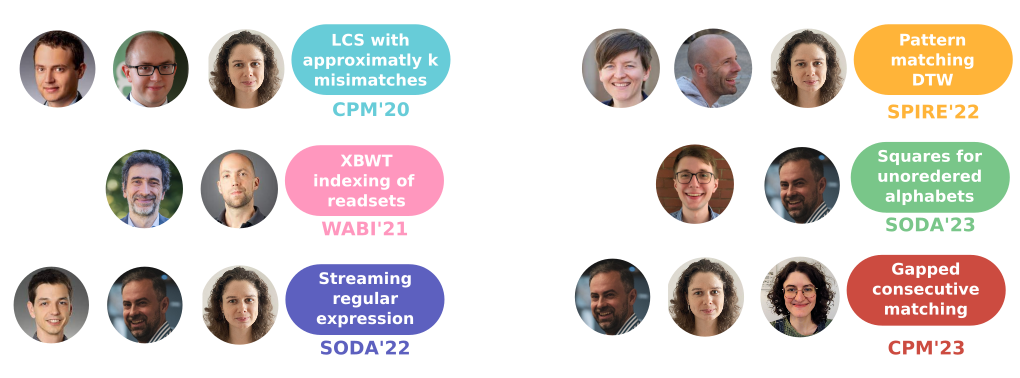
\includegraphics[width=\textwidth]{pictures/mindmap/co_auth.png}
\end{frame}

\begin{frame}[noframenumbering,plain]
  \centering
  \only<1|handout:0>{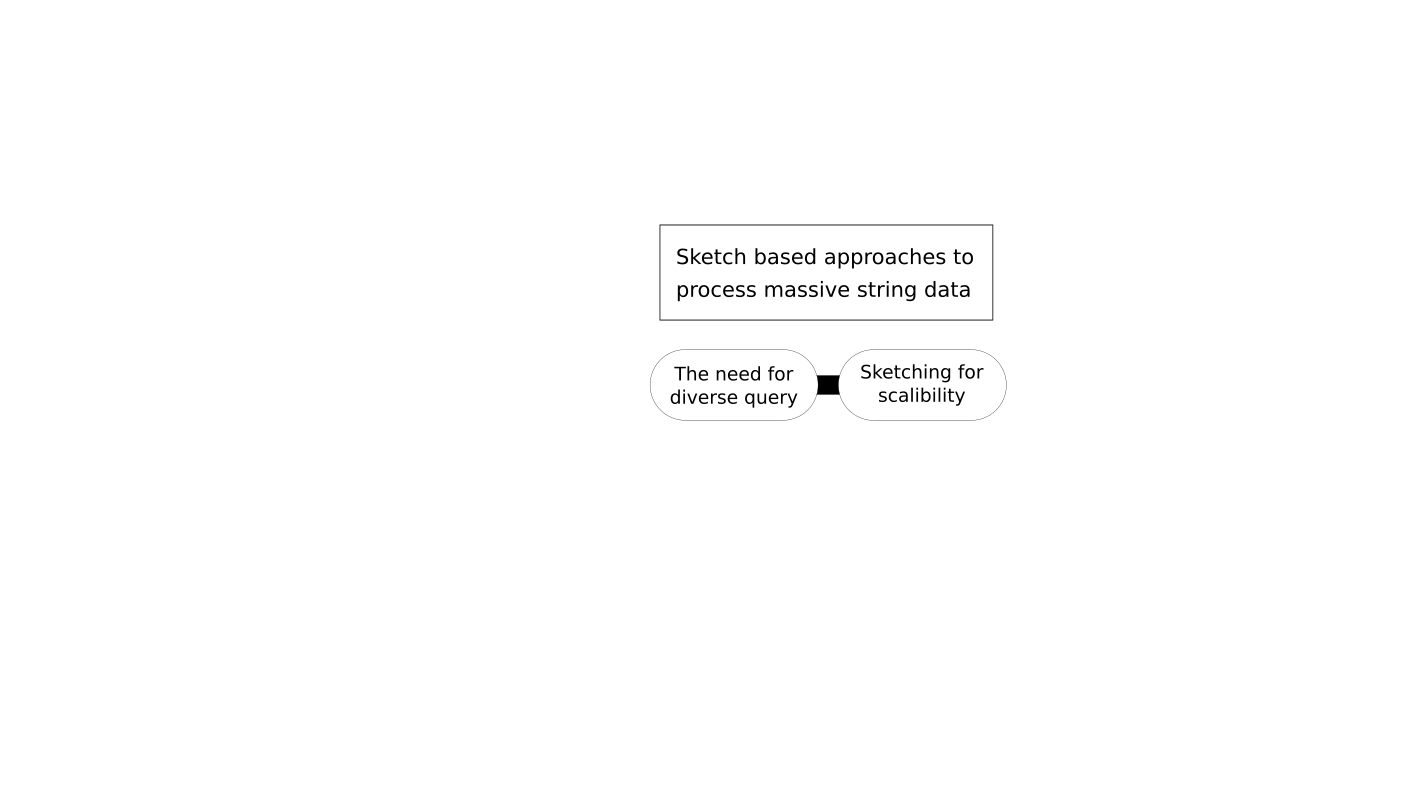
\includegraphics[width=0.5\textwidth]{pictures/mindmap/1.png}}
  \only<2|handout:0>{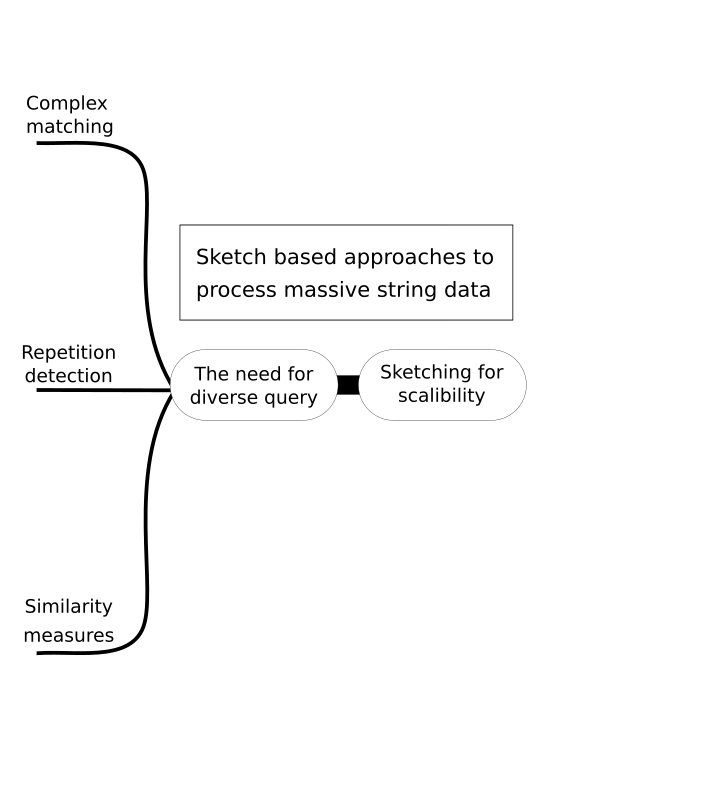
\includegraphics[width=0.5\textwidth]{pictures/mindmap/2.png}}
  \only<3|handout:0>{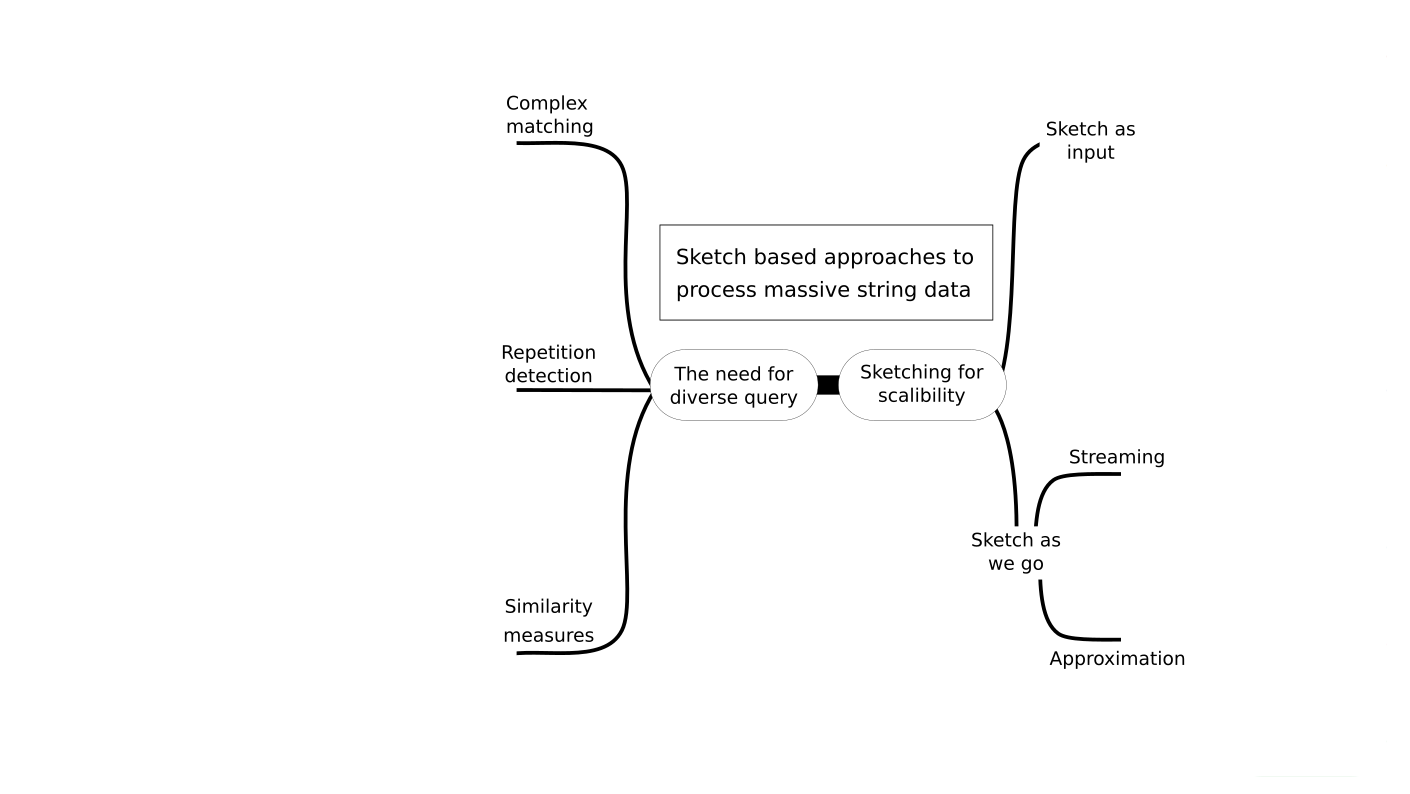
\includegraphics[width=\textwidth]{pictures/mindmap/3b.png}}
  \only<4|handout:0>{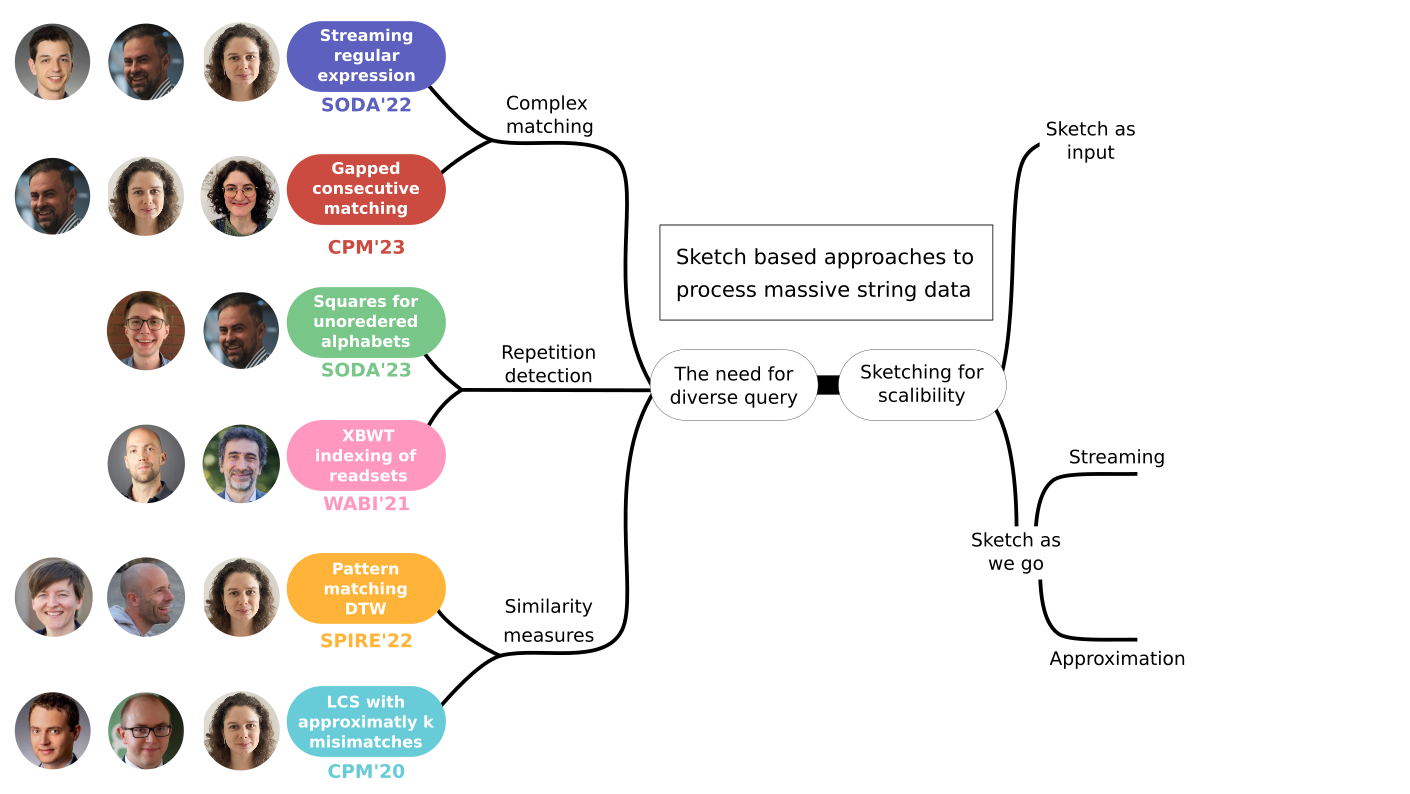
\includegraphics[width=\textwidth]{pictures/mindmap/4.png}}
  \only<5|handout:0>{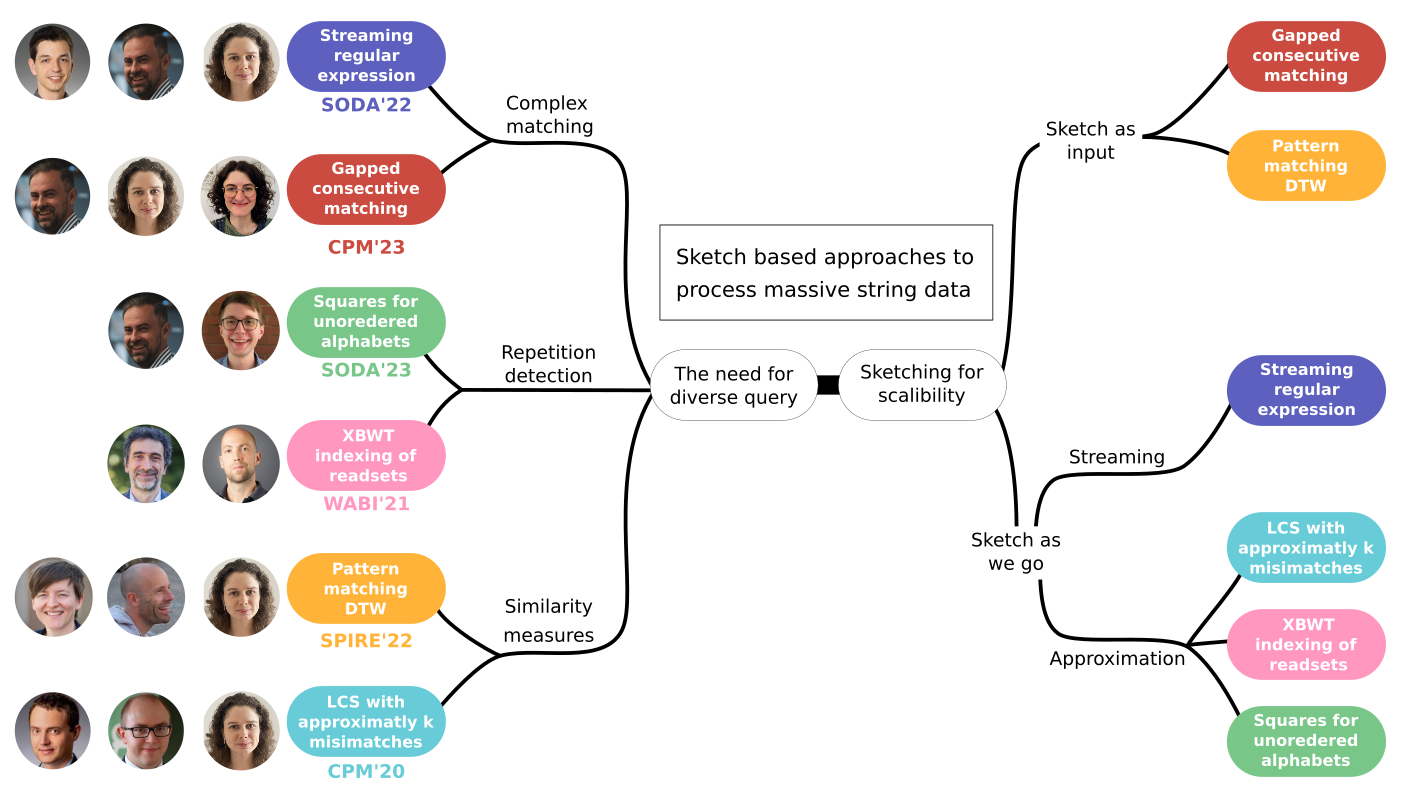
\includegraphics[width=\textwidth]{pictures/mindmap/5.png}}
  \only<6>{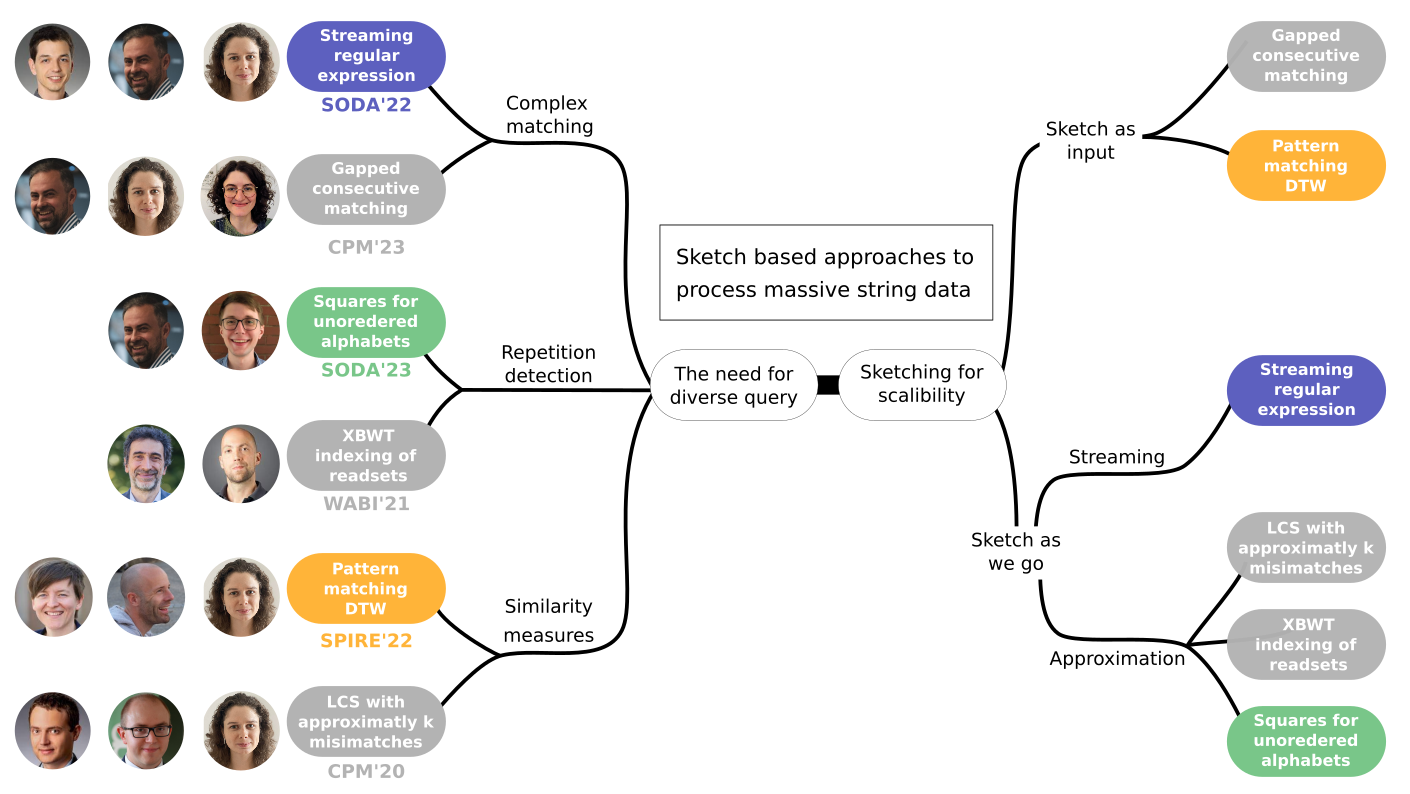
\includegraphics[width=\textwidth]{pictures/mindmap/present.png}}
\end{frame}


\subsection{Regular Expressions in Streaming}
\begin{frame}
  \centering
  {\Large Streaming Regular Expression Membership and Pattern Matching}

  \bigskip
  {\large SODA'22}\\
  \bigskip
  
\includegraphics{pictures/mindmap/regexp.png}

  \bigskip
  Bartłomiej Dudek, Paweł Gawrychowski, Tatiana Starikovskaya
\end{frame}

\begin{frame}{A powerful matching model: regular expressions}
    \begin{columns}
        \column{.6\textwidth}
        \begin{mydefblock}{Regular expressions (regexp)}
            either a character from $\Sigma$ or recursively defined from other regular expressions $R_1$ and $R_2$:
            %\pause
            \begin{enumerate}
                \item $R_1 \cdot R_2$ (concatenation),
                %\pause
                \item $R_1 | R_2$ (union),
                %\pause
                \item $R_1^\ast$ (Kleene star).
            \end{enumerate}
        \end{mydefblock}
        \pause
        \column{.4\textwidth}
        \begin{center}
            %\only<1|handout:0>{\textbf{Ex:} For $\Sigma=\{a,b\}$,\\ 
            % $R_1=a$ only matches $a$,\\
            % and $R_2=b$ only matches $b$.}
            %\only<2|handout:0>{$R_1 \cdot R_2$ matches anything matching $R_1$ followed by anything matching $R_2$.\\
            %\textbf{Ex:} with $R_1=a$ and $R_2=b$, $R_1 \cdot R_2$ matches $ab$.}
            %\only<3|handout:0>{$R_1 | R_2$ matches anything matching $R_1$ or  $R_2$.\\
            %\textbf{Ex:} with $R_1=a \cdot b = ab$ and $R_2=b$, $R_1 | R_2$ matches $ab$ and $b$.}
            %\only<4|handout:0>{$R_1^\ast$ matches any number of repetition of any string matching $R_1$.\\
            %\textbf{Ex:} with $R_1=(b|ab)$ matches $\varepsilon$, $ab$, $b$, $bbabb$...}
            %\only<5->{
                \textbf{Ex:} $b(b|ab)^\ast ab$\\
                \smallskip
                \cmark ~ $bbbbbabab$ \\
                \cmark ~ $bbbabbbbab$\\
                \xmark ~ $bbbaabbbab$\\
                \xmark ~ $baba$\\ 
                \xmark ~ $abab$\\
            %    }
        \end{center}
    \end{columns}    
    %\pause
    %\pause

    \bigskip
    Used in databases, \pause data mining, \pause secret detection, \pause computer networks, \pause protein search\pause ...\\
    \pause
    \bigskip
    {
        \beamermathcolor{myblue}
        Given a regular expression $R$ and a string $T$, \bblue{membership} is : check if $R$ matches $T$.\\
        %\bblue{Pattern matching:} check if $R$ matches \textbf{some substring} of $T$. \pause \\
        %\textcolor{myblue}{Reduces to membership!}
    }
    
    
    \pause
    \medskip
    We define the length of $R$ to be the number of $\cdot$, $|$, and $\ast$ that it contains.
\end{frame}

\begin{frame}{A frugal model of computation: Streaming}
\begin{columns}
    \column{.4\textwidth}
    The algorithm first receives and preprocesses the expression.\\ Next, it keeps reading characters from a very very long string and:
    \column{.5\textwidth}
    \begin{center}
        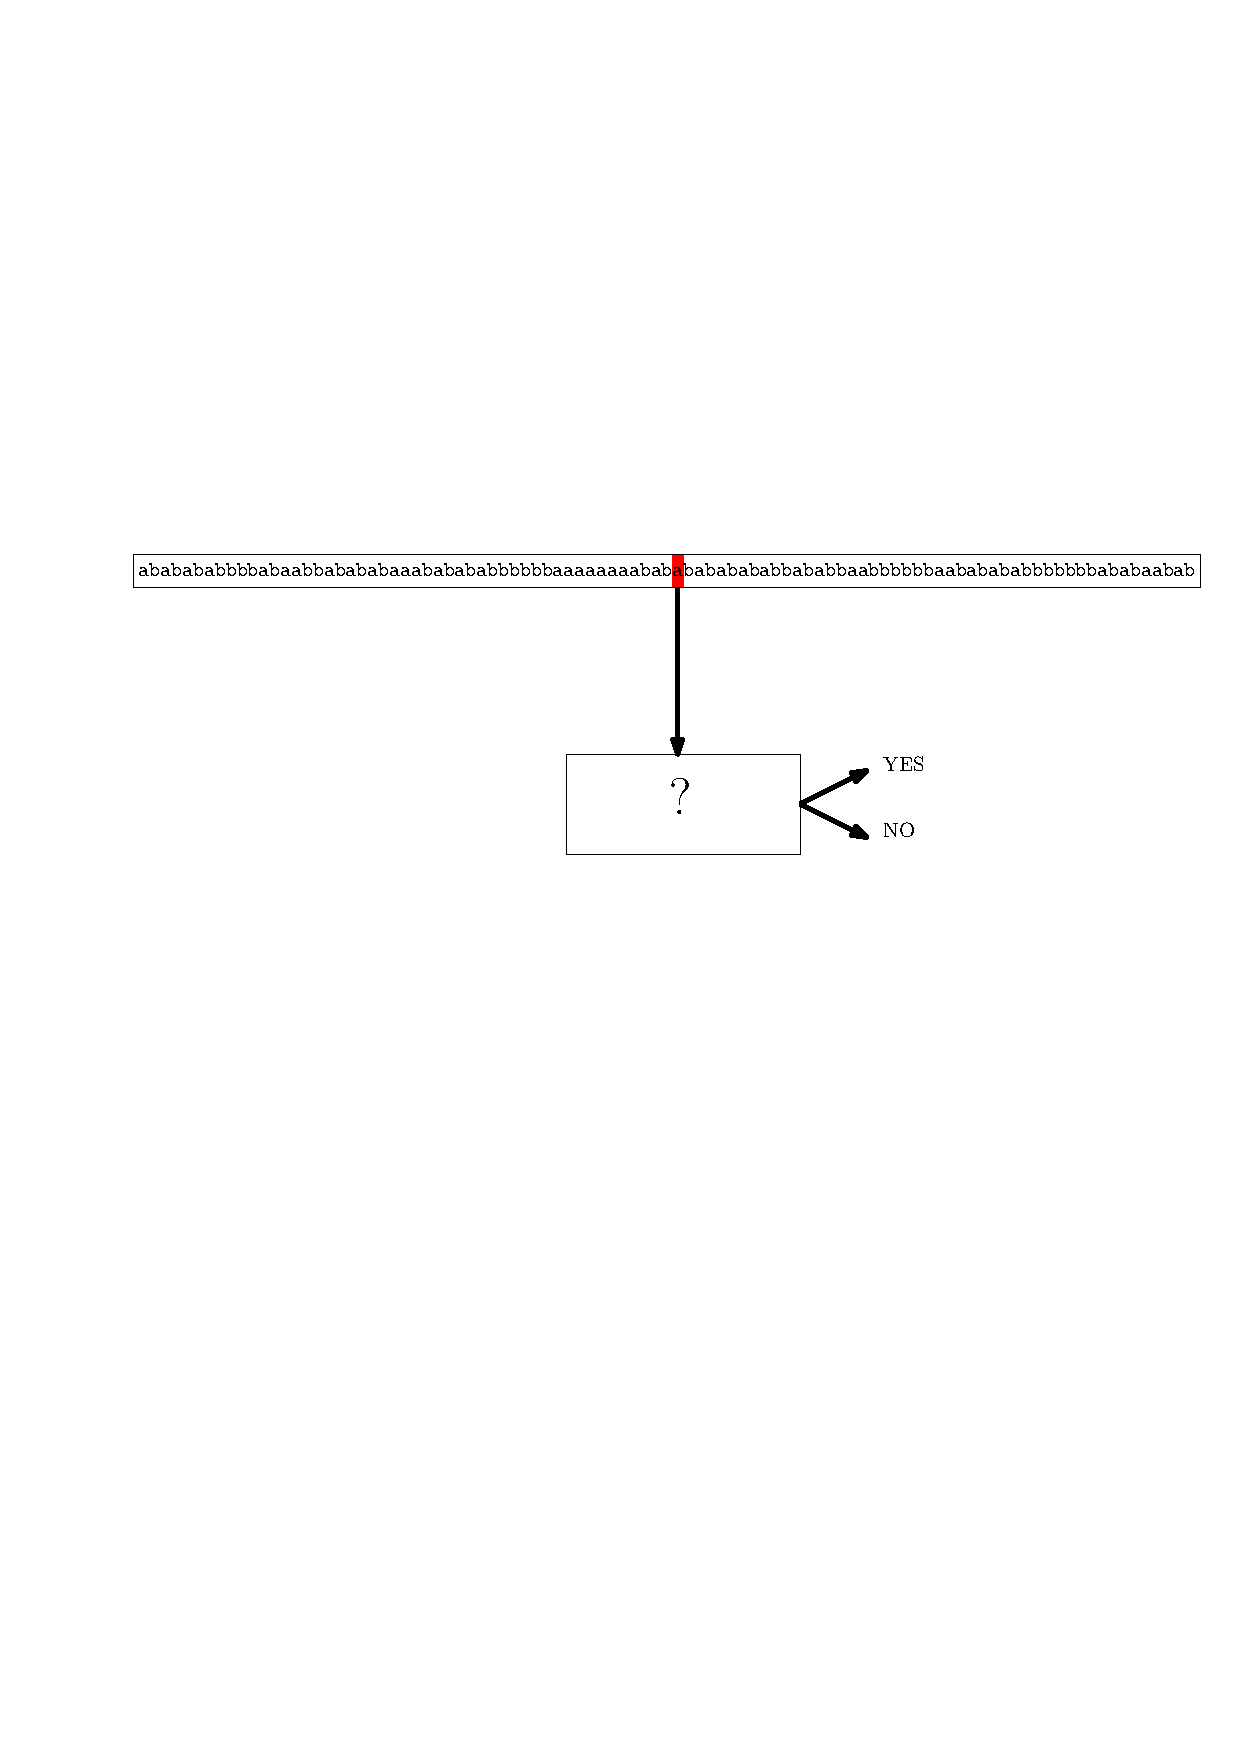
\includegraphics[width=\textwidth]{pictures/stream3}
    \end{center}
\end{columns}

\smallskip
\pause
\begin{enumerate}
\item \textbf{No delay:} After having seen the $i$-th character, immediately report whether the string so far matches the regular expression.
\pause
\item \textbf{No going back:} Not possible to read any of the earlier characters.
\pause
\item \textbf{Every space counts:} No access to the original expression (unless stored explicitly).
\end{enumerate}
\pause
\begin{center}
    \small
    A crucial  tool is the variant of Karp--Rabin fingerprints of \ntheme{[Porat and Porat, FOCS'09]}.
\end{center}\pause
\begin{mylemblock}{Classic pattern matching in streaming [Breslauer and Galil, TALG'14]}
    For a pattern of length $m$, it takes $\Oh(\log m)$ space and $\Oh(1)$ time per position.
\end{mylemblock}

\end{frame}

\begin{frame}{State of the art on regular expression membership}
    \begin{columns}
        \column{.4\textwidth}
        For a regexp of length $m$,\\
        \ntheme{Classic:} Recursively build the \btheme{Thompson automata}, then check if $T$ is accepted.\\
        $\Oh(m)$ space and time/character.
        \column{.5\textwidth}
        \centering
        \begin{picture}(200,65)
            \put(0,0){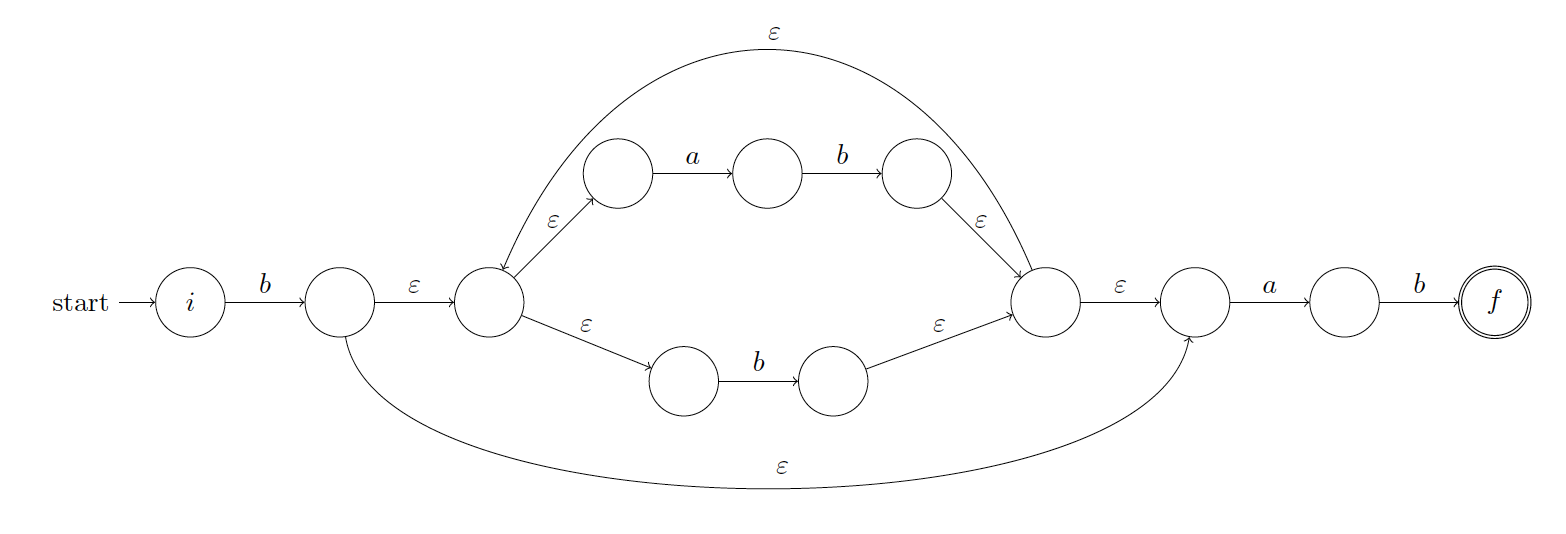
\includegraphics[width=\textwidth]{pictures/thomson1.png}}
            \put(150,50){\small $b(b|ab)^\ast ab$}
        \end{picture}
    \end{columns}
    \pause
    \medskip
    \begin{itemize}
        \setlength{\itemsep}{2ex}
        \item The best improvements on the time complexity \ntheme{only reduce by logarithmic factors}.\pause
        \item Fine-grained complexity proved conditional lowerbounds, with \ntheme{``hard to match'' expressions} where \textcolor{red}{improvements are unlikely}.\pause
        \item \ntheme{[Bille and Thorup, SODA'10]} $\Oh((\frac{d\log w}{w}+\log d))$ time/character and $\Oh(m)$ space, where $d$ is the number of occurrences of $|$ and $\ast$, and $w$ is the word size.\pause
    \end{itemize}
    \vfill
    \begin{center} What about \textcolor{red}{\textbf{space efficiency}} ? 
    \end{center}
\end{frame}

{\renewcommand{\arraystretch}{2}
\begin{frame}{Space-efficiency for regular expression}
    For a regexp of length $m$, $O(m)$ space for the Thompson automata, can we do better ? \pause

    \medskip
    \textbf{Some intuition:} \ntheme{other problems studied in streaming} \pause

    \medskip
    \begin{tabular}{l c p{0.25\textwidth}}
        Problem & Translation to regular expressions & Space complexity\\ 
        \hline \pause
        Dictionary matching & $(P_{1}|\ldots | P_{d})$ & $\Oh(d\log m)$  \mbox{\footnotesize [Golan~and~Porat~ESA'17]}\\ \pause
        Wildcards matching & $P_{1}(1|\ldots|\sigma)P_{2}\ldots P_{d}(1|\ldots|\sigma)P_{d+1}$ & $\Oh(d\log m)$ \mbox{\footnotesize [Golan et al.,~Algorithmica'19]} \pause
    \end{tabular}

    \medskip
    \begin{myalertblock}{Dudek, Gawrychowski, Gourdel, Starikovskaya, SODA'22}
        For any regular expression $R$ with $d$ occurrences of $|$ and $\ast$, we can solve regular expression membership on a string of length $n$ using $\Oh(d^{3}\polylog n)$ space and $\Oh(nd^{5}\polylog n)$ time per character.
    \end{myalertblock}
\end{frame}
}

\begin{frame}{Summary}
    \textbf{Complex matching:} regular expression, one of the most powerful and versatile model.

    \vfill
    
    \textbf{Sketch as we go: streaming} Karp-Rabin fingerprints as a space efficient way to keep information on the stream.

    \begin{myalertblock}{Dudek, Gawrychowski, Gourdel, Starikovskaya, SODA'22}
        For any regular expression $R$ with $d$ occurrences of $|$ and $\ast$, we can solve regular expression membership on a string of length $n$ using $\Oh(d^{3}\polylog n)$ space and $\Oh(nd^{5}\polylog n)$ time per character.
    \end{myalertblock}
    \vfill
    \textbf{Not shown:} Technical part, Witness mechanism, circuit machinery.
\end{frame}
\section{Pattern Matching DTW}

\newcommand{\dtw}{\mathrm{DTW}}
\newcommand{\ed}{\mathrm{ED}}
\newcommand{\RLE}{\mathrm{RLE}}


\begin{frame}
    \centering
    {\Large Optimal Square Detection  Over General Alphabets}
  
    \bigskip
    {\large SPIRE'22}\\
    \bigskip
    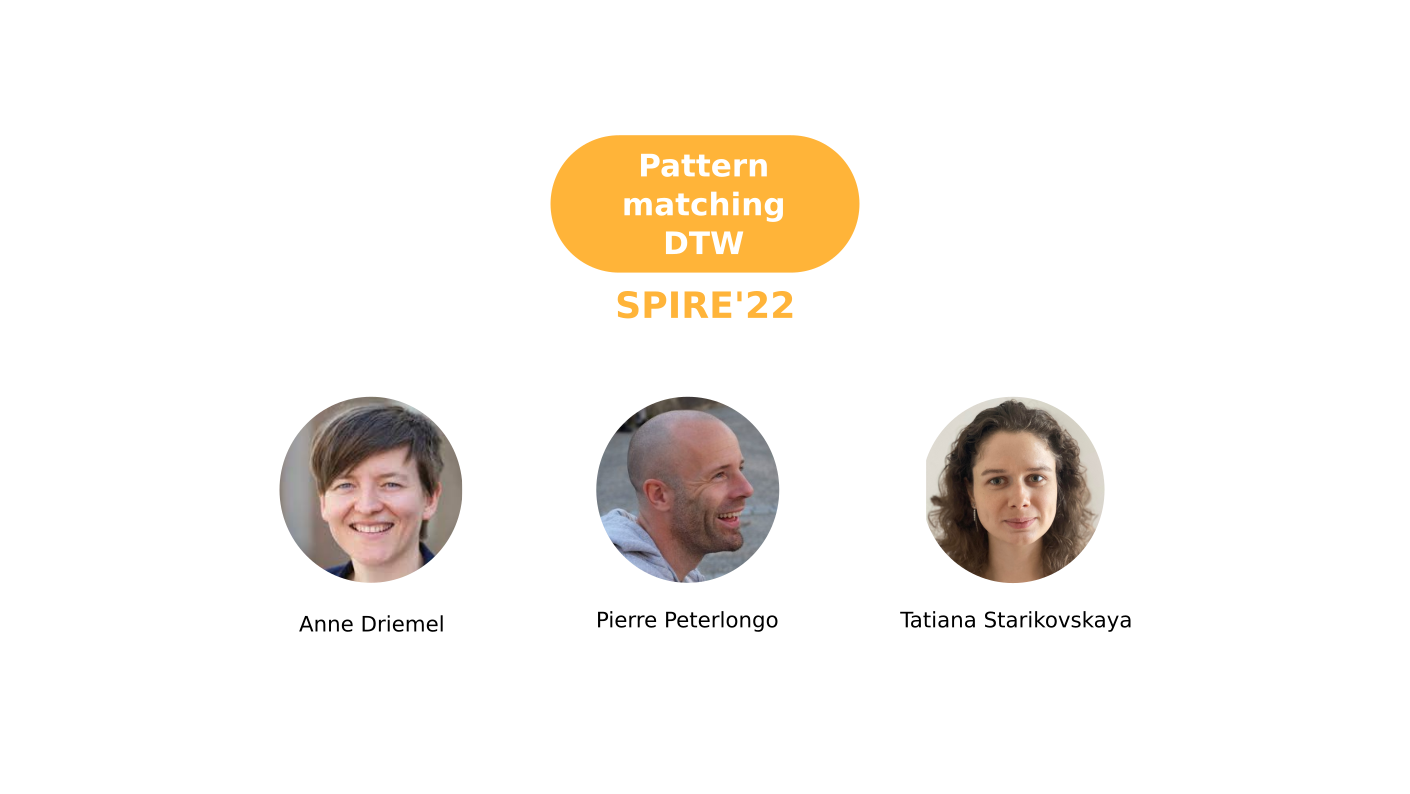
\includegraphics{pictures/mindmap/dtw.png}
  
    \bigskip
    Anne Driemel, Pierre Peterlongo, Tatiana Starikovskaya
\end{frame}


\begin{frame}{Dynamic time warping (DTW) distance: comparing time series}

\btheme{Definition:} Minimal distance obtained by \ntheme{duplicating} some items (maintaining equal length) and then \ntheme{summing the distances} between items at the same position.

\begin{center}
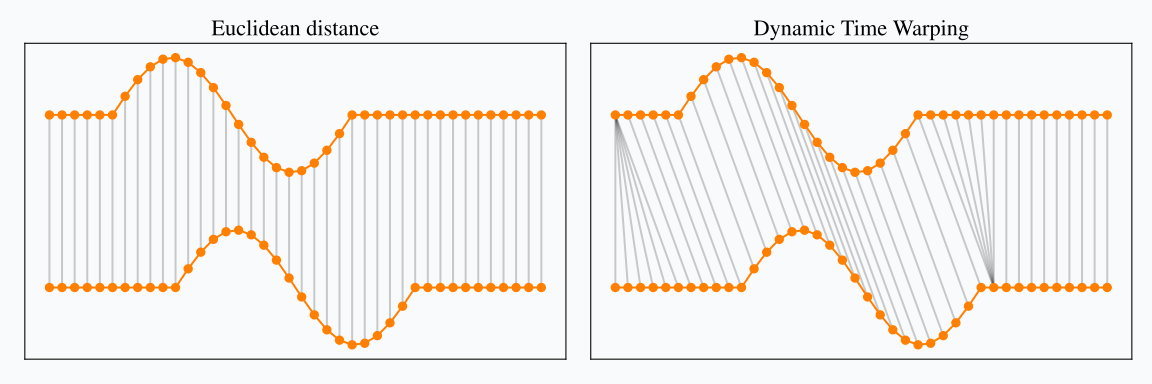
\includegraphics[scale=0.3]{figures/dtw_vs_euc.png}\\
\tiny{Figure credit: Romain Tavenard}
\end{center}
\pause
\small
Used in \ntheme{speech recognition} to deal with varying speeds and more generally for parametrized curves where each item is a \ntheme{multidimensional point}.\pause

\vfill
But what about \btheme{strings} where the items are characters from $\Sigma$ (finite) ?
\end{frame}

\begin{frame}{Dynamic Time Warping (DTW) Distance for Strings }

\begin{columns}
\column{0.5\textwidth}
Given $X$ and $Y$ strings, $\dtw(X,Y)$ is the
minimal distance obtained by \ntheme{duplicating} some characters (maintaining equal length) and then \ntheme{summing the distances} between characters at the same position.
\vfill
\column{0.4\textwidth}

\only<2>{
\begin{mdframed}
\center
{\tiny Distance between characters = hamming distance.} 
\footnotesize
\begin{figure}
%\missingfigure{Under construction...}
\centering
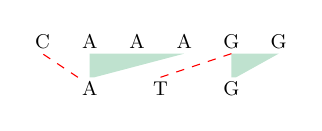
\begin{tikzpicture}[scale=0.6, every node/.style={scale=0.8}]
\foreach \x[count=\i] in {C,A,A,A,G,G} {
    \node at ($(\i, 1)$) {\small{\x}};
}
\foreach \y[count=\j] in {A,T,G} {
    \node at ($(0.5+\j*1.5, 0)$) {\small{\y}};
}
% align A
\fill[mygreen!25] (2, 0.25) -- (2,0.75) -- (4,0.75) -- (2.1,0.25) -- cycle;
% align G
\fill[mygreen!25] (5, 0.25) -- (5,0.75) -- (6,0.75) -- (5.1,0.25) -- cycle;
%draw misalignment
\draw[dashed,red] (1.75, 0.25) -- (1,0.75);
\draw[dashed,red] (3.5, 0.25) -- (5,0.75);
\end{tikzpicture}
\end{figure}
\vfill 
$\dtw($CAAAG$,$ATG$)=2$\\
\end{mdframed}}

\end{columns}
\pause


\only<3->{

\btheme{Dynamic Programming}\\
\smallskip
$D$ a matrix of size $(|X|+1)(|Y|+1)$ such that $D[i,j]=\dtw(X[1..i],Y[1..j])$\pause
\bigskip

\btheme{Initialization}~~~$D[0,0]= 0$ and for all $(i,j)$, $D[0,j]=D[i,0]=+\infty$.\\
\pause
\bigskip
\btheme{Recurrence} ~~~ 
    $D[i,j] = \min\{$\beamermathcolor{black}
        $\underbrace{\mathcolor{black!30!blue}{D[i-1,j-1]}}_\text{top-left},
        \underbrace{\mathcolor{black!30!blue}{D[i-1,j]}}_\text{top},
        \underbrace{\mathcolor{black!30!blue}{D[i,j-1]}}_\text{left}$
    $\mathcolor{black!30!blue}{\}+ d(X[i], Y[j])}$.
}

\end{frame}


\begin{frame}{Why is DTW on strings interesting ? Third generation sequencing}
    \small
    When DNA is sequence, we obtain fragments (reads) of the DNA that have to be assembled.
    \begin{columns}
    \column{0.4\textwidth}
    \smallskip
    \btheme{Third generation sequencing}\\
    \smallskip
    \textcolor{mygreen}{Long reads, fast and portable.}\\
    \smallskip
    \textcolor{red}{Higher error rate.}\\
    \smallskip
    Uneven speed of the DNA through the nanopore, creates errors on the length when the same nucleotide is repeated (homopolymers/runs)...
    \column{0.5\textwidth}
    \begin{center}
    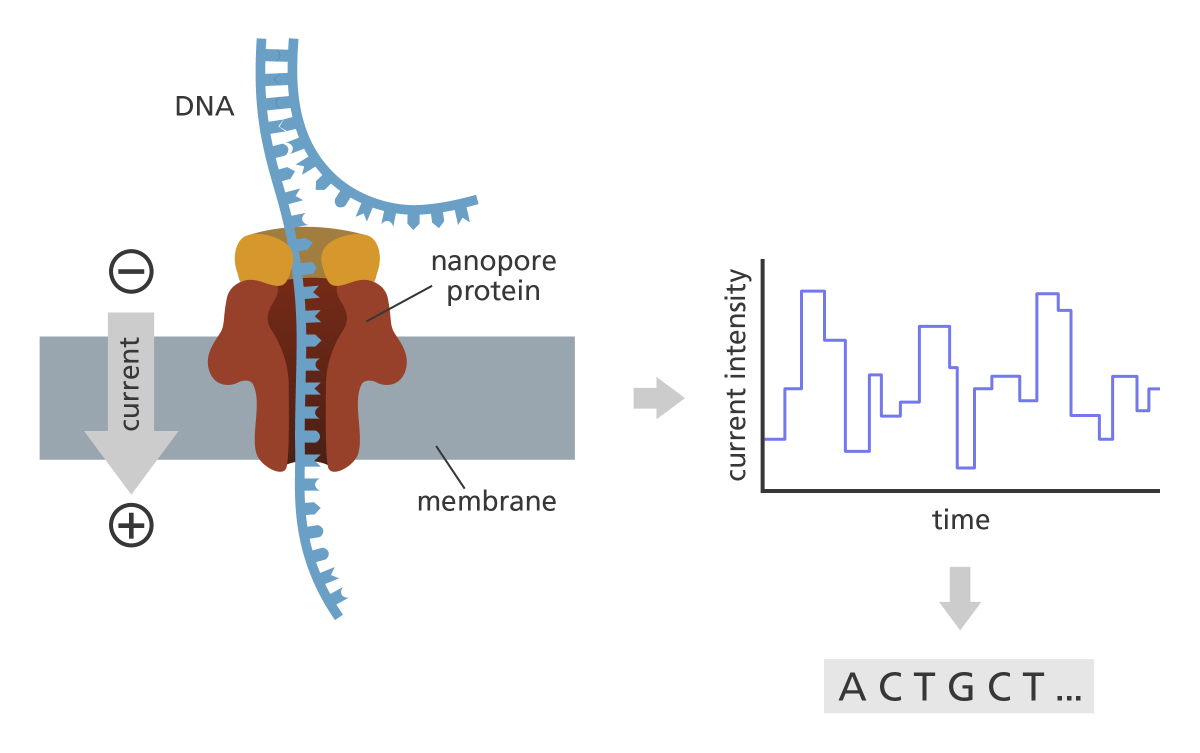
\includegraphics[scale=0.20]{figures/ont-sequencing_yourgenome.png}\\
    {\tiny Figure credit: \href{https://www.yourgenome.org/facts/what-is-oxford-nanopore-technology-ont-sequencing/}{yourgenome.org}}
    \end{center}
    
    \end{columns}
    \vfill
    { DTW  was already used to \ntheme{align the raw signal} by [Loose et al. 2016] and [Han et al. 2020].\\
    We propose to use it to \ntheme{align the reads (strings)} to a reference (string).\\ 
    So we want to find the position where it aligns best ($\neq$ similarity btw. two strings) ?}
    
\end{frame}

\begin{frame}{Our subject: Pattern Matching for DTW}

    \begin{columns}
    \column{0.45\textwidth}
    \begin{mydefblock}{Pattern matching DTW}
        \btheme{Input}~~two strings $P$ and $T$.\\ 
        \btheme{Output}~~for every $0 \leq j < |T|$, 
        ~~~$\min_{0 \leq i \leq j} \dtw(P,T[i..j])$.
    \end{mydefblock}
    
    \column{0.4\textwidth}
    \vfill
    \btheme{Dynamic Programming}\\
    \smallskip
    \ntheme{Changes the Initialization}\\
    for all $0\leq j\leq |T|$, $D[0,j]= 0$ and 
    for all $1 \leq i \leq |P|$, $D[i,0]=+\infty$.\\
    \vfill
    \end{columns}
    \pause
    
    \bigskip
    
    
    \begin{center}
        
\begin{center}
\footnotesize
\resizebox{0.8\textwidth}{!}{
\begin{tabular}{|cc||cc|cccc|c|cc|c|cccc|cc|c|c|c|c|c|}
\hline
 &   & G & G & T & T & T & T & C & T & T & A & T & T & T & T & G & G & T & G & A & T & A \\
 & 0 & 0 & 0 & 0 & \textcolor{red}{0} & 0 & 0 & 0 & 0 & 0 & 0 & 0 & 0 & 0 & 0 & 0 & 0 & 0 & 0 & 0 & 0 & 0 \\
\hline
A  & $\infty$  & 1 & 1 & 1 & 1 & \textcolor{red}{1} & 1 & 1 & 1 & 1 &{ 0 } & 1 & 1 & 1 & 1 & 1 & 1 & 1 & 1 &{ 0 } & 1 &{ 0 }\\
A  & $\infty$  & 2 & 2 & 2 & 2 & 2 & \textcolor{red}{2} & 2 & 2 & 2 &{ 0 } & 1 & 2 & 2 & 2 & 2 & 2 & 2 & 2 &{ 0 } & 1 &{ 0 }\\
\hline
T  & $\infty$  & 3 & 3 &{ 2 } &{ 2 } &{ 2 } &{ 2 } & \textcolor{red}{3} &{{ 2 }} &{{ 2 }} & 1 &{ 0 } &{ 0 } &{ 0 } &{ 0 } & 1 & 2 &{ 2 } & 3 & 1 &{ 0 } & 1\\
T  & $\infty$  & 4 & 4 &{ 2 } &{ 2 } &{ 2 } &{ 2 } & 3 & \textcolor{red}{{ 2 }} &{{ 2 }} & 2 &{ 0 } &{ 0 } &{ 0 } &{ 0 } & 1 & 2 &{ 2 } & 3 & 2 &{ 0 } & 1\\
\hline
A  & $\infty$  & 5 & 5 & 3 & 3 & 3 & 3 & 3 & 3 & \textcolor{red}{3} &{{ 2 }} & 1 & 1 & 1 & 1 & 1 & 2 & 3 & 3 &{ 2 } & 1 &{ 0 }\\
\hline
T  & $\infty$  & 6 & 6 &{ 3 } &{ 3 } &{ 3 } &{ 3 } & 4 &{ 3 } &{ 3 } & \textcolor{red}{3} &{{ 1 }} &{{ 1 }} &{{ 1 }} &{{ 1 }} & 2 & 2 &{ 2 } & 3 & 3 &{ 1 } & 1\\
\hline

\end{tabular} }
\end{center}



\pause
        \medskip
        \small{\textcolor{red}{Diagonals can be non-monotone.}}
    \end{center}
    
\end{frame}


\begin{frame}{State of the art for DTW on strings}
    $X$ and $Y$ strings, $N=|X|$ and $M=|Y|$.
    \only<3->{With $n$ and $m$ runs in $X$ and $Y$.}\\
    \smallskip
    The dynamic programming takes $\Oh(NM)$ time $=\Oh(N^2)$ in the case $N=M$.\\ \pause
    \begin{block}{No strongly subquadratic [Gold and Sharir]}
    %There are no strongly subquadratic algorithms to compute the DTW distance between two strings over a ternary alphabet unless the Strong Exponential Hypothesis (SETH) is false.
    $|\Sigma| \geq 3 \Rightarrow $ no $\Oh(N^{a})$ time algorithm with $a<2$ unless SETH is false.
    \end{block}\pause

    \ntheme{Run-length compressed} \\
    $\dtw(X,Y)$ can be computed $\Oh(mN+Mn)$-time [Froese et al.] 
    
    \smallskip
    \ntheme{Low distance regime}\\
    If $\dtw(X,Y) \leq k$ it can be computed in $\Oh(kN)$-time [Kuszmaul]
    
    \medskip

    \textcolor{red}{Can we also use (and combine) those approaches for Pattern Matching ?}

\end{frame}

\begin{frame}{Runs simplify the dynamic programming matrix}
    $T$ and $P$ strings, $N=|T|$ and $M=|P|$, with $n$ and $m$ runs. \pause
    \smallskip

    We call $D[i_p .. j_p, i_t .. j_t]$ a \btheme{\emph{block}} if $P[i_p.. j_p]$ is a run in $P$, and $T[i_t .. j_t]$ is a run in $T$.
    
    
    %
\begin{center}
\footnotesize
\resizebox{0.8\textwidth}{!}{
\begin{tabular}{|cc||cc|cccc|c|cc|c|cccc|cc|c|c|c|c|c|}
\hline
 &   & G & G & T & T & T & T & C & T & T & A & T & T & T & T & G & G & T & G & A & T & A \\
 & 0 & 0 & 0 & 0 & {0} & 0 & 0 & 0 & 0 & 0 & 0 & 0 & 0 & 0 & 0 & 0 & 0 & 0 & 0 & 0 & 0 & 0 \\
\hline
A  & $\infty$  & 1 & 1 & \textcolor{red}{1} & \textcolor{red}{1} & \textcolor{red}{1} & \textcolor{red}{1} & 1 & 1 & 1 &{ 0 } & 1 & 1 & 1 & 1 & 1 & 1 & 1 & 1 &{ 0 } & 1 &{ 0 }\\
A  & $\infty$  & 2 & 2 & \textcolor{red}{2} & \textcolor{red}{2} & \textcolor{red}{2} & \textcolor{red}{2} & 2 & 2 & 2 &{ 0 } & 1 & 2 & 2 & 2 & 2 & 2 & 2 & 2 &{ 0 } & 1 &{ 0 }\\
\hline
T  & $\infty$  & 3 & 3 &{ 2 } &{ 2 } &{ 2 } &{ 2 } & {3} &{{ 2 }} &{{ 2 }} & 1 &{ 0 } &{ 0 } &{ 0 } &{ 0 } & 1 & 2 &{ 2 } & 3 & 1 &{ 0 } & 1\\
T  & $\infty$  & 4 & 4 &{ 2 } &{ 2 } &{ 2 } &{ 2 } & 3 & {{ 2 }} &{{ 2 }} & 2 &{ 0 } &{ 0 } &{ 0 } &{ 0 } & 1 & 2 &{ 2 } & 3 & 2 &{ 0 } & 1\\
\hline
A  & $\infty$  & 5 & 5 & 3 & 3 & 3 & 3 & 3 & 3 & {3} &{{ 2 }} & 1 & 1 & 1 & 1 & 1 & 2 & 3 & 3 &{ 2 } & 1 &{ 0 }\\
\hline
T  & $\infty$  & 6 & 6 &{ 3 } &{ 3 } &{ 3 } &{ 3 } & 4 &{ 3 } &{ 3 } &{3} &{{ 1 }} &{{ 1 }} &{{ 1 }} &{{ 1 }} & 2 & 2 &{ 2 } & 3 & 3 &{ 1 } & 1\\
\hline

\end{tabular} }
\end{center}




    {\beamermathcolor{black}
    \[
        D[i,j] = {\min\{D[i-1,j-1],D[i-1,j],D[i,j-1]\}
        + \underbrace{d(X[i], Y[j])}_\text{\textcolor{red}{Constant inside a block!}}}
    \]
    }
            
    Inside a block, the values are \ntheme{non-decreasing along a row/column/diagonal}.
    We can take the shortest path inside a block $\rightarrow$ $\Oh(Nm+Mn)$ time.\\
    If $d$ is an integer distance, the values $\leq k$ can take \ntheme{at most $k$ distinct values}...
    
    \begin{myalertblock}{Driemel, Gourdel, Peterlongo, Starikovskaya}
        For an \textcolor{red}{integer} distance $d: \Sigma \times \Sigma \rightarrow \mathbb{Z}^+$, given $P$ and $T$ run-length compressed with $m$ and $n$ runs resp.,
        we can compute all $\dtw$ distances $\leq k$ in $\Oh(k mn)$ time.
    \end{myalertblock}
    \end{frame}

\begin{frame}{Summary}
    \textbf{Similarity measure:} the Dynamic Time Warping distance on string can be used to align reads with homopolymers errors onto a reference genome.

    \vfill
    
    \textbf{Sketch as input:} Run-length compression sketch, suited to the metric, that allows a complexity proportional to the size of the sketch not the original input.
    
    \vfill
    \begin{myalertblock}{Driemel, Gourdel, Peterlongo, Starikovskaya}
        For an \textcolor{red}{integer} distance $d: \Sigma \times \Sigma \rightarrow \mathbb{Z}^+$, given $P$ and $T$ run-length compressed with $m$ and $n$ runs resp.,
        we can compute all $\dtw$ distances $\leq k$ in $\Oh(k mn)$ time.
    \end{myalertblock}
    \vfill
    \textbf{Not shown:} $\Oh(n+m)$ algorithm for $k=1$, \ntheme{approximations}  results and \ntheme{experiments}.
\end{frame}
    

\section{Squares for Unordered Alphabets}
\newcommand{\absolute}[1]{\left\lvert#1\right\rvert}
\newcommand{\orderof}[1]{\mathcal{O}(#1)}

\begin{frame}
    \centering
    {\Large Optimal Square Detection  Over General Alphabets}
  
    \bigskip
    {\large SODA'23}\\
    \bigskip
    
\includegraphics{pictures/mindmap/squares.png}
  
    \bigskip
    Jonas Ellert, Paweł Gawrychowski
  \end{frame}

\begin{frame}{Squares and repetition detection}

\end{frame}


\begin{frame}{Alphabet types for $w \in \Sigma^n$, where $|\Sigma| = \sigma$}
    \small
	\vspace{.75\baselineskip}	
	
	\setlength{\leftmargini}{1.1em}
	\begin{itemize}
	\onslide<2->{\item \textbf{linearly-sortable alphabet (LSA)}:\hfill \hspace{0.5cm}%
	\onslide<3->{e.g.\ $\{\texttt A,\texttt C,\texttt G,\texttt T\}$, $\{0, \dots, 255\}$, or $\{1, \dots, n^{\Oh({1})}\}$}
	\\sort $n$ symbols in $\Oh({n})$ time%\\e.g.\ $\{1, \dots, n^{\Oh{1}}\}$%
	}
	\vspace{.25\baselineskip}
	\onslide<4->{\item \textbf{general ordered alphabet (GOA)}:\hfill %
	\onslide<5->{\rlap{e.g.\ comparison sort}\phantom{e.g.\ $\{\texttt A,\texttt C,\texttt G,\texttt T\}$, $\{0, \dots, 255\}$, or $\{1, \dots, n^{\Oh{1}}\}$}}
	\\test $w[i] < w[j]$ in constant time}
	\vspace{.25\baselineskip}
	\onslide<6->{\item \textbf{general unordered alphabet (GUA)}:\hfill%
	\onslide<7->{\rlap{e.g.\ KMP pattern matching}\phantom{e.g.\ $\{\texttt A,\texttt C,\texttt G,\texttt T\}$, $\{0, \dots, 255\}$, or $\{1, \dots, n^{\Oh{1}}\}$}}
	\\test $w[i] = w[j]$ in constant time}
	\end{itemize}
	
	\vspace{1.5\baselineskip}
	\onslide<8->
	\begin{tabular}{r|ccc} 
		& LSA & GOA & GUA \\\hline
		%${}^{\strut}$Element Distinctness & $\Theta(\sigma)$ & $\Theta(\sigma \lg \sigma)$ & $\Theta(\sigma^2)$ \pause \\
		$\strut^{\strut}$Lempel-Ziv & %
		\onslide<9->{$\Oh({n})$} & %
		\onslide<10->{$\Theta(n \lg \sigma)$} & %
		\onslide<11->{$\Theta(n\sigma)$} \\ %
		%
		$\strut$Suffix Sorting & %
		\onslide<9->{$\Oh({n})$} & %
		\onslide<10->{$\Theta(n \lg \sigma)$} & %
		\onslide<11->{$\Theta(n\sigma)$} \\
		%
		\onslide<12->{${}^{\strut}$\bfseries Square-Freeness} & %
		\onslide<12->{\boldmath$\Oh({n})$\unboldmath} & %
		\onslide<13->{\boldmath$\Theta(n)$\unboldmath} & %
		\onslide<14->{\boldmath$\Oh(n \lg n)$\unboldmath} \begin{tikzoverlay}
			\onslide<15->{
            \beamermathcolor{black}
			\tikzset{viscol1/.style={white}}
			\tikzset{viscol2/.style={white}}
			\tikzset{viscol3/.style={white}}
			\only<16->{\tikzset{viscol1/.style={}}}
			\only<17->{\tikzset{viscol2/.style={}}}
			\only<17->{\tikzset{viscol3/.style={red}}}
			\path (0,.1) node (a) {};
			\draw (3,1.1) node (b) {optimal for $\sigma = n$};
			\node[below=-.4em of b,viscol1] (c) {but what about $\sigma < n\strut$?};
			\node[below=-.0em of c,viscol2] (d) {{\boldmath$\Theta(n \lg \sigma)$\unboldmath}};
			\node[below=-.4em of d,viscol3] (e) {\textbf{\small Our contribution}};
			\node[fit=(b)(c)(d)(e), ultra thick, draw=red, inner sep=.25em] (f) {};			
			\draw[-latex] (f.west |- b.center) to[out=180, in=0] (a);
			}
		\end{tikzoverlay} \\
		%
		${}^{\strut}$ & %
		\onslide<12->{\footnotesize\bfseries\color{red} Kolpakov \&} & %
		\onslide<13->{\footnotesize\bfseries\color{red} Ellert \&} & %
		\onslide<14->{\footnotesize\bfseries\color{red} e.g.\ Main \&} \\
		& %
		\onslide<12->{\footnotesize\bfseries\color{red} Kucherov '99} & %
		\onslide<13->{\footnotesize\bfseries\color{red} Fischer '21} & %
		\onslide<14->{\footnotesize\bfseries\color{red} Lorentz '84}
	\end{tabular}	
	
\end{frame}

\begin{frame}{The use of Lempel-Ziv factorization to detect squares}
    
\end{frame}

\begin{frame}
\frametitle{Sketching: $\Delta$-approximate Lempel-Ziv factorisation}
\vspace{.5\baselineskip}


\onslide<2->{\textbf{\boldmath$\Delta$\unboldmath-approximate Lempel-Ziv factorisation:} $w = f_1f_2\dots f_z$}\onslide<4->{ such that}
\begin{itemize}
\item<4-> $\absolute{f_i} > 0$ and $f_i = h_it_i$ (\emph{head} and \emph{tail}) with $\absolute{h_i} < \Delta$\onslide<6->{, and}
\item<6-> $t_i$ is empty or occurs at least twice in $f_1f_2\dots f_i$\onslide<8->{, and}
\item<8-> $f_if_{i + 1}[1]$ does not occur in $f_1f_2\dots f_i$ (or $i = z$).
\end{itemize}

\vspace{.5\baselineskip}

\onslide<3->
\begin{center}
\begin{tikzpicture}
\tikzset{barcolor/.style={black, densely dotted}}
\tikzset{fcolor/.style={black}}

\setcounter{symbid}{0}
\foreach[count=\factorid from 1, evaluate=\factorid as \prevfid using int(\factorid-1)] \factorset in {%
{a,b},%
{c,b,a,b},%
{a,a,b,c,b,a},%
{c,b,a,b,a,a,b,c},%
{z,z,b,a,b,a}%
}
{

\only<5->{
\ifnum\factorid=4
	\tikzset{barcolor/.style={black, densely dotted}}
	\tikzset{fcolor/.style={black, font=\boldmath}}	
\else
    \beamermathcolor{black!30!white}
	\tikzset{barcolor/.style={black!30!white, densely dotted}}
	\tikzset{fcolor/.style={barcolor}}
\fi}

\path (\thesymbid\lzspacing+0.5\lzspacing, -0.5em) node (leftbar) {};
\foreach \tsymb in \factorset {
	\addtocounter{symbid}{1}
	\node[inner sep=0] (\thesymbid) at (\thesymbid\lzspacing,0) {\smash{\texttt{\tsymb}\vphantom{$\strut$}}$\vphantom{m}$};
	%\node at (\thesymbid\lzspacing,1) {$\scriptstyle\thesymbid$};
}
\path (\thesymbid\lzspacing+0.5\lzspacing, -0.5em) node (rightbar) {};
\path (leftbar) to node[midway] (centerbar) {} (rightbar);
\node[above=.75em of centerbar |- \thesymbid.north, fcolor] (flab\factorid) {$f_{\factorid}$};

\ifodd\factorid\else
	\draw[thick, barcolor] (leftbar.center) to ++(0,1);
	\draw[thick, barcolor] (rightbar.center) to ++(0,1);
\fi
}

\foreach[count=\i from 13, evaluate=\i as \j using int(\i-10)] \x in {c,b} {
\node<5->[below=1em of \i, inner sep=0] (low\i) {\smash{\texttt{\x}\vphantom{$\strut$}}$\vphantom{m}$};
\node<10->[below=1em of \j, inner sep=0] (low\j) {\smash{\texttt{\x}\vphantom{$\strut$}}$\vphantom{m}$};
}

\foreach[count=\i from 15, evaluate=\i as \j using int(\i-10)] \x in {a,b,a,a,b,c} {
\node<5->[below=1em of \i, inner sep=0] (low\i) {\smash{\texttt{\x}\vphantom{$\strut$}}$\vphantom{m}$};
\node<7->[below=1em of \j, inner sep=0] (low\j) {\smash{\texttt{\x}\vphantom{$\strut$}}$\vphantom{m}$};
}

\tikzset{hlbox/.style={draw, ultra thick, inner xsep=2.5pt}}

\only<5->{
\node[hlbox, fit=(low13)(low14), red] (h4) {};
\node[hlbox, fit=(low15)(low20), myorange] (t4) {};

\node[below=0 of h4] (h4lab) {$h_4$};
\node[below=0 of t4] (t4lab) {$t_4$};

\draw[thick, barcolor] (h4.south west) ++(0, -0.002em) to (h4.west |- h4lab.south);
\draw[thick, barcolor] (h4.south east) ++(0, -0.002em) to (h4.east |- h4lab.south);
\draw[thick, barcolor] (t4.south east) ++(0, -0.002em) to (t4.east |- h4lab.south);

}

\node<10->[hlbox, fit=(low3)(low4), red] {};
\node<7->[hlbox, fit=(low5)(low10), myorange] {};

\onslide<8->{
\node<9->[below=1em of 21, inner sep=0] (low21) {\smash{\texttt{z}\vphantom{$\strut$}}$\vphantom{m}$};
\node<11->[below=1em of 11, inner sep=0] (low11) {\smash{\texttt{b}\vphantom{$\strut$}}$\vphantom{m}$};
\node<9->[hlbox, fit=(low21), mygreen] {};
\node<11->[hlbox, fit=(low11), myblue] {};
}

\only<14->{
\node[hlbox, fit=(17)] {};
\node[hlbox, fit=(18)] {};

\node<15->[hlbox, fit=(7)] {};
\node<15->[hlbox, fit=(8)] {};
}

\draw node[left=0 of 1] {$w = \strut$};
\node<5->[right=6em of t4lab] {$\Delta = 3$};

\end{tikzpicture}
\end{center}

\vspace{.25\baselineskip}

\begin{itemize}
%\item<9-> if $f_i[1..\absolute{f_i})$ overlaps its earlier occurrence, then square already found
\item<13-> no need to detect squares that are entirely contained in $t_i$
\end{itemize}

\onslide<12->
\begin{mylemblock}{\textbf{Lemma}}
\begin{tikzpicture}[overlay, remember picture]
\node (mark) {};
\end{tikzpicture}
{\small $\frac\strut\strut$A $\Delta$-approximate LZ factorisation can be computed in $\orderof{n + \frac{n \cdot \lg n \cdot \sigma}{\sqrt{\Delta}}}$ time.}
\end{mylemblock}

\end{frame}

\begin{frame}{Using our sketch to detect squares}

\begin{center}
    \small

    \begin{tikzpicture}[scale=0.9, every node/.style={transform shape}]
    \beamermathcolor{black}
    \onslide<2->{
    
    \node (0) {$\qquad\quad w = {}$};
    \foreach[evaluate=\i as \iminus using int(\i-1)] \i in {1,...,30} {
        \node[right=0 of \iminus, minimum width=1.05em] (\i) {\vphantom{a}};
        \node[below=-0.75em of \i, minimum width=1.05em] (d\i) {\vphantom{a}};
    }
    
    
    \node[fit=(1)(30), fill=white, draw=black, inner sep=0pt] {};
    \node[fit=(6)(15), fill=myblue!40!white, inner sep=0pt] (larm) {};
    \node[fit=(16)(25), fill=myblue!40!white, inner sep=0pt] (rarm) {};
    \node at (larm.center) {$\alpha$};
    \node at (rarm.center) {$\alpha$};
    
    \node[fit=(1)(30), draw=black, inner sep=0pt] {};
    \node[fit=(6)(15), thick, draw=black, inner sep=0pt] (larm) {};
    \node[fit=(16)(25), thick, draw=black, inner sep=0pt] (rarm) {};
    
    \tikzset{barcolor/.style={densely dotted}}
    \tikzset{fcolor/.style={}}
    
    \onslide<3->{
    
    \foreach[%
    evaluate=\len as \lensum using int(\prevlensum+\len), %
    evaluate=\prevlensum as \starti using int(\prevlensum+1),
    remember=\lensum as \prevlensum initially 0,
    count=\j from 1] %
    \len in {1,2,4,6,5,5,7} {
    
        \node[fit=(\starti)(\lensum), inner sep=0pt] (fact\j) {};
    
        \only<4->{
        \ifnum\j=6
            \tikzset{fcolor/.style={font=\boldmath}}
        \else
            \beamermathcolor{black!30!white}
            \tikzset{barcolor/.style={black!30!white, densely dotted}}
            \tikzset{fcolor/.style={black!30!white}}
        \fi}
        
        \node[above=0.25em of fact\j, fcolor] (flab\j) {$f_{\j}$};
        
        \ifodd\j\else\ifnum\j=6
            \draw<-3>[thick, barcolor] (fact\j.south west) ++(0,-.002) to ++(0,1.002);
            \draw<-3>[thick, barcolor] (fact\j.south east) ++(0,-.002) to ++(0,1.002);
        \else
            \draw[thick, barcolor] (fact\j.south west) ++(0,-.002) to ++(0,1.002);
            \draw[thick, barcolor] (fact\j.south east) ++(0,-.002) to ++(0,1.002);
        \fi\fi
    }
    
    \onslide<4->{
    \node[fit=(d19)(d20), thick, fill=red!50!white, draw=black, inner sep=0pt] (rhead) {};
    \node[fit=(d21)(d23), thick, fill=myorange!50!white, draw=black, inner sep=0pt] (rfac) {};
    \node[fit=(d24.north west)(d24.south), thick, fill=mygreen!50!white, draw=black, inner sep=0pt] (rnext) {};
    \node at (rhead.center) {$h_6$};
    \node at (rfac.center) {$t_6$};
    \draw[thick, barcolor] (fact6.south west) ++(0,1) to (fact6.west |- rfac.south);
    \draw[thick, barcolor] (fact6.south east) ++(0,1) to (fact6.east |- rfac.south);
    }
    
    \onslide<5->{
    \node[fit=(d9)(d10), thick, fill=red!50!white, draw=black, inner sep=0pt] (lhead) {};
    \node[fit=(d11)(d13), thick, fill=myorange!50!white, draw=black, inner sep=0pt] (lfac) {};
    \node[fit=(d14.north west)(d14.south), thick, fill=mygreen!50!white, draw=black, inner sep=0pt] (lnext) {};
    \node at (lhead.center) {$h_6$};
    \node at (lfac.center) {$t_6$};
    %\draw[thick, barcolor] (lfac.west |- larm.north) to (lfac.south west);
    %\draw[thick, barcolor] (lfac.east |- larm.north) to (lfac.south east);
    }
    
    \onslide<6->{\node [right=0em of flab6, red] {\LARGE\xmark};}
    
    }}
    
    \end{tikzpicture}
    \end{center}
    
    \vspace{-.5\baselineskip}
    
    \begin{itemize}
    \item<7-> The right arm of square intersects at most two factors.
    \item<8-> Squares that are larger than $\geq 8\Delta$ intersect at least a tail of length $\geq \Delta$.
    \item<9-> We can use the Main+Lorentz'84 to detect in $\Oh(n)$ time any such squares.
    \item<10-> For squares $\leq 8\Delta$, we slice the text into overlapping small blocks.
    \end{itemize}

    
    \begin{center}
    \begin{tikzpicture}[scale=0.85, every node/.style={transform shape}]
    
    \node (0) {$w = {}$};
    \foreach[evaluate=\i as \iminus using int(\i-1)] \i in {1,...,30} {
        \node[right=0 of \iminus, minimum width=1.05em] (\i) {\vphantom{a}};
        \node[below=0em of \i, minimum width=1.05em] (d\i) {\vphantom{a}};
    }
    
    \foreach[
    evaluate=\x as \firstx using int((\x-1)*5+1),
    evaluate=\x as \lastx using int(\x*5),
    ] \x in {1,...,6} {
    \beamermathcolor{black}
    \node[fit=(\firstx)(\lastx), draw, inner sep=0pt] (x\x) {};
    \node at (x\x) {$B_{\x}$};
    }
    
    \node[fit=(d1)(d5)] {\leftarrowfill};
    \node[fit=(d1)(d5)] (lenmark) {\rightarrowfill};
    \node[below=0 of lenmark.center] {$\Theta(\Delta)$};
    
    
    \pause\node[above=-.2em of x1.north east] (firstpair) {$\overbrace{\hspace{10.25em}}^{\text{$\orderof{\Delta \lg \Delta}$ time}}$};
    %\node[above right=.25 and -.5 of firstpair] (fpnote) {\small $\text{algorithm by \textcolor{red}{\bfseries Main+Lorentz'84}}$};
    %\draw[-latex] (fpnote) to[out=180, in=90] (firstpair);
    \pause\node[below=-.2em of x2.south east] {$\underbrace{\hspace{10.25em}}_{\text{$\orderof{\Delta \lg \Delta}$ time}}$};
    \pause\node[above=-.2em of x3.north east] {$\overbrace{\hspace{10.25em}}^{\text{$\orderof{\Delta \lg \Delta}$ time}}$};
    \pause\node[below=-.2em of x4.south east] {$\underbrace{\hspace{10.25em}}_{\text{$\orderof{\Delta \lg \Delta}$ time}}$};
    \pause\node[above=-.2em of x5.north east] {$\overbrace{\hspace{10.25em}}^{\text{$\orderof{\Delta \lg \Delta}$ time}}$};
    
    \pause
    
    \end{tikzpicture}
    
    \vspace{1.0\baselineskip}
    \small
    \onslide<9->{$\implies$ Choose $\Delta = (\sigma \lg n)^2$ to achieve $\orderof{n (\lg \sigma + \lg \lg n)}$ time.}
    \onslide<10->{But we cannot know $\sigma$...\\}
    \end{center}
    \smallskip
    \onslide<11->{\small We proceed in $\log \log n$ phases, with decreasing $\Delta_i$, detecting ``long'' squares until we see that the alphabet is too large and we can ``afford'' $\Oh(n\log \Delta_i)$ 
    + Amortization across the levels.  }
\end{frame}

\begin{frame}{Summary}
    \textbf{Repetition detection:} 
    \vfill
    
    \textbf{Sketch:} 
    \vfill
    \begin{myalertblock}{}
    \end{myalertblock}
    \vfill
    \textbf{Not shown:} .
\end{frame}
    

\section{Conclusion}
\begin{frame}
  \vfill
  \mytitle{Conclusion}
  \bigskip
  \begin{center}
    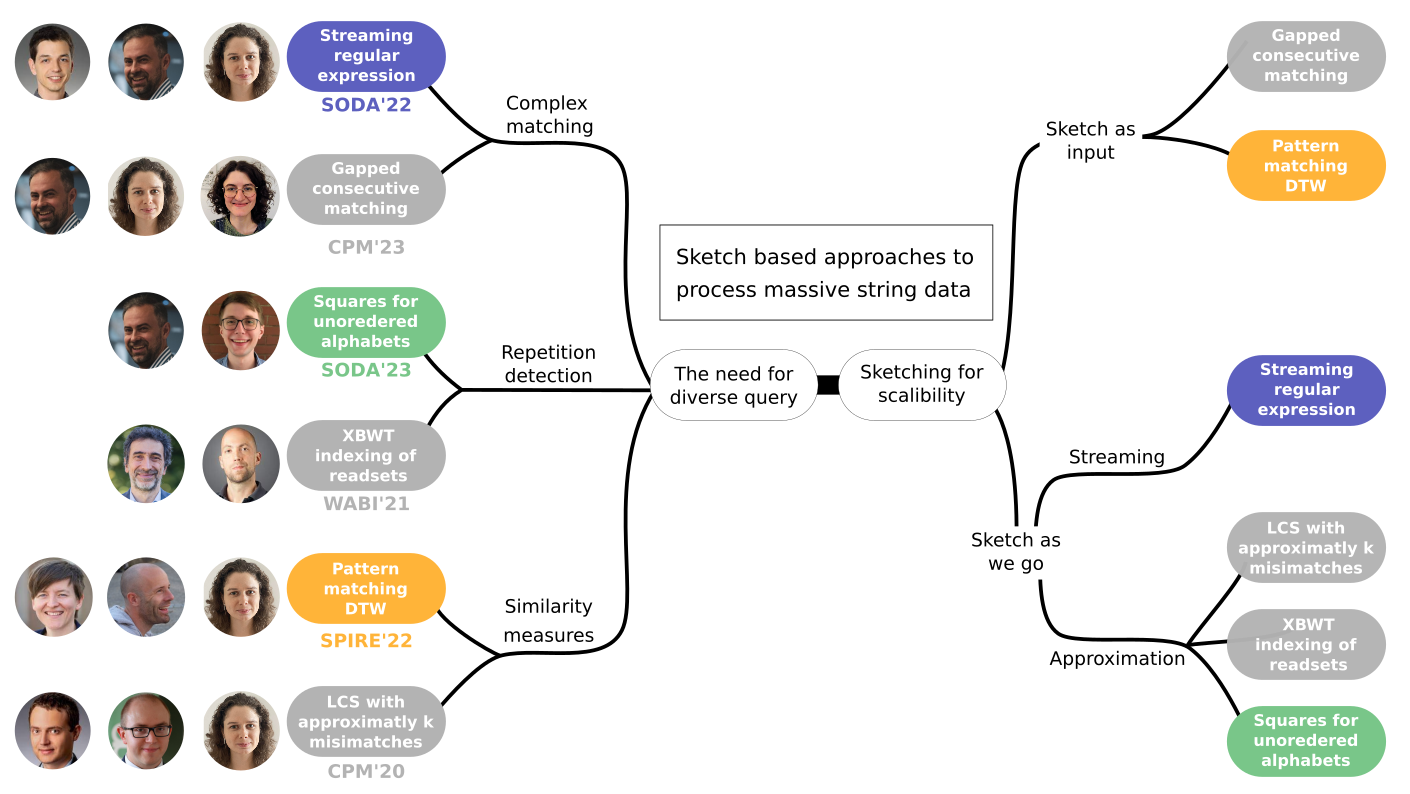
\includegraphics[width=0.8\textwidth]{pictures/mindmap/present.png}
  \end{center}
  \vfill
\end{frame}

\begin{frame}
  \begin{center}
    \mytitle{Conclusion}
  \end{center}
  \btheme{Main thesis:} Sketches can enable fast and space-efficient algorithms!

  \medskip
  \btheme{Open questions:}
  \begin{itemize}
    \item \ntheme{Streaming regular expressions:} improve the time complexity while still maintaining space $\sim \mathrm{poly}(d,\log n)$? Improving space complexity?
    \item \ntheme{Pattern matching for the Dynamic Time Warping distance:} faster algorithms? \textcolor{gray}{[Boneh et al. arxiv'23]} Is $\tilde{\Oh}(k(n+m))$ space and time possible?
    \item \ntheme{Squares over general alphabets:} adapt the lowerbound to randomized algorithms ?
  \end{itemize}

  \medskip
  \btheme{Larger perspectives:} applications of the sketches in practice, with a special interest on Lempel-Ziv scheme that are widely used in practice for their low memory usage when constructing the factorization.
\end{frame}

\backupbegin
\begin{frame}[noframenumbering,plain]
  \vfill
  \mytitle{Thank you !}
  \bigskip
  \begin{center}
    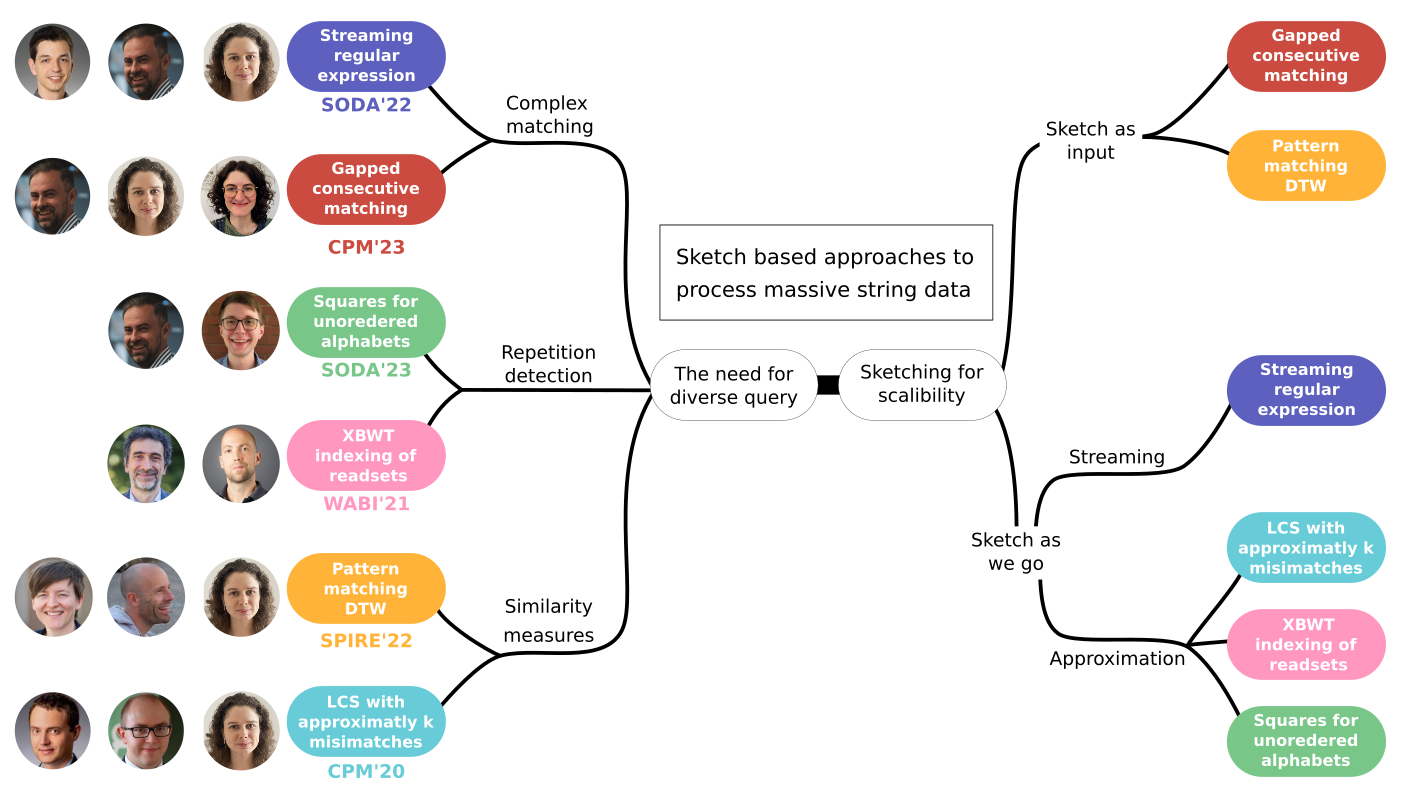
\includegraphics[width=0.8\textwidth]{pictures/mindmap/5.png}
  \end{center}
  \vfill
\end{frame}

\appendix
\backupbegin

\section{Gapped consecutive matching}

\begin{frame}
  \centering
  {\Large Gapped Consecutive Matching}

  \bigskip
  \begin{minipage}{0.55\textwidth}  
    \begin{enumerate}
      \item Grammar Compressed Indexing (CPM'23)
      \item Grammar Compressed Pattern Matching
    \end{enumerate}
  \end{minipage}\\
  \bigskip
  
  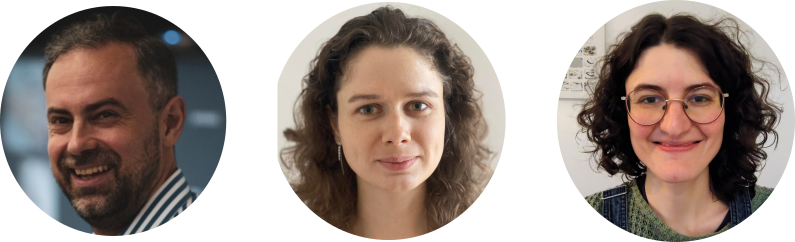
\includegraphics{pictures/mindmap/gapped.png}

  \bigskip
  Paweł Gawrychowski, Tatiana Starikovskaya, Teresa Anna Steiner
\end{frame}


%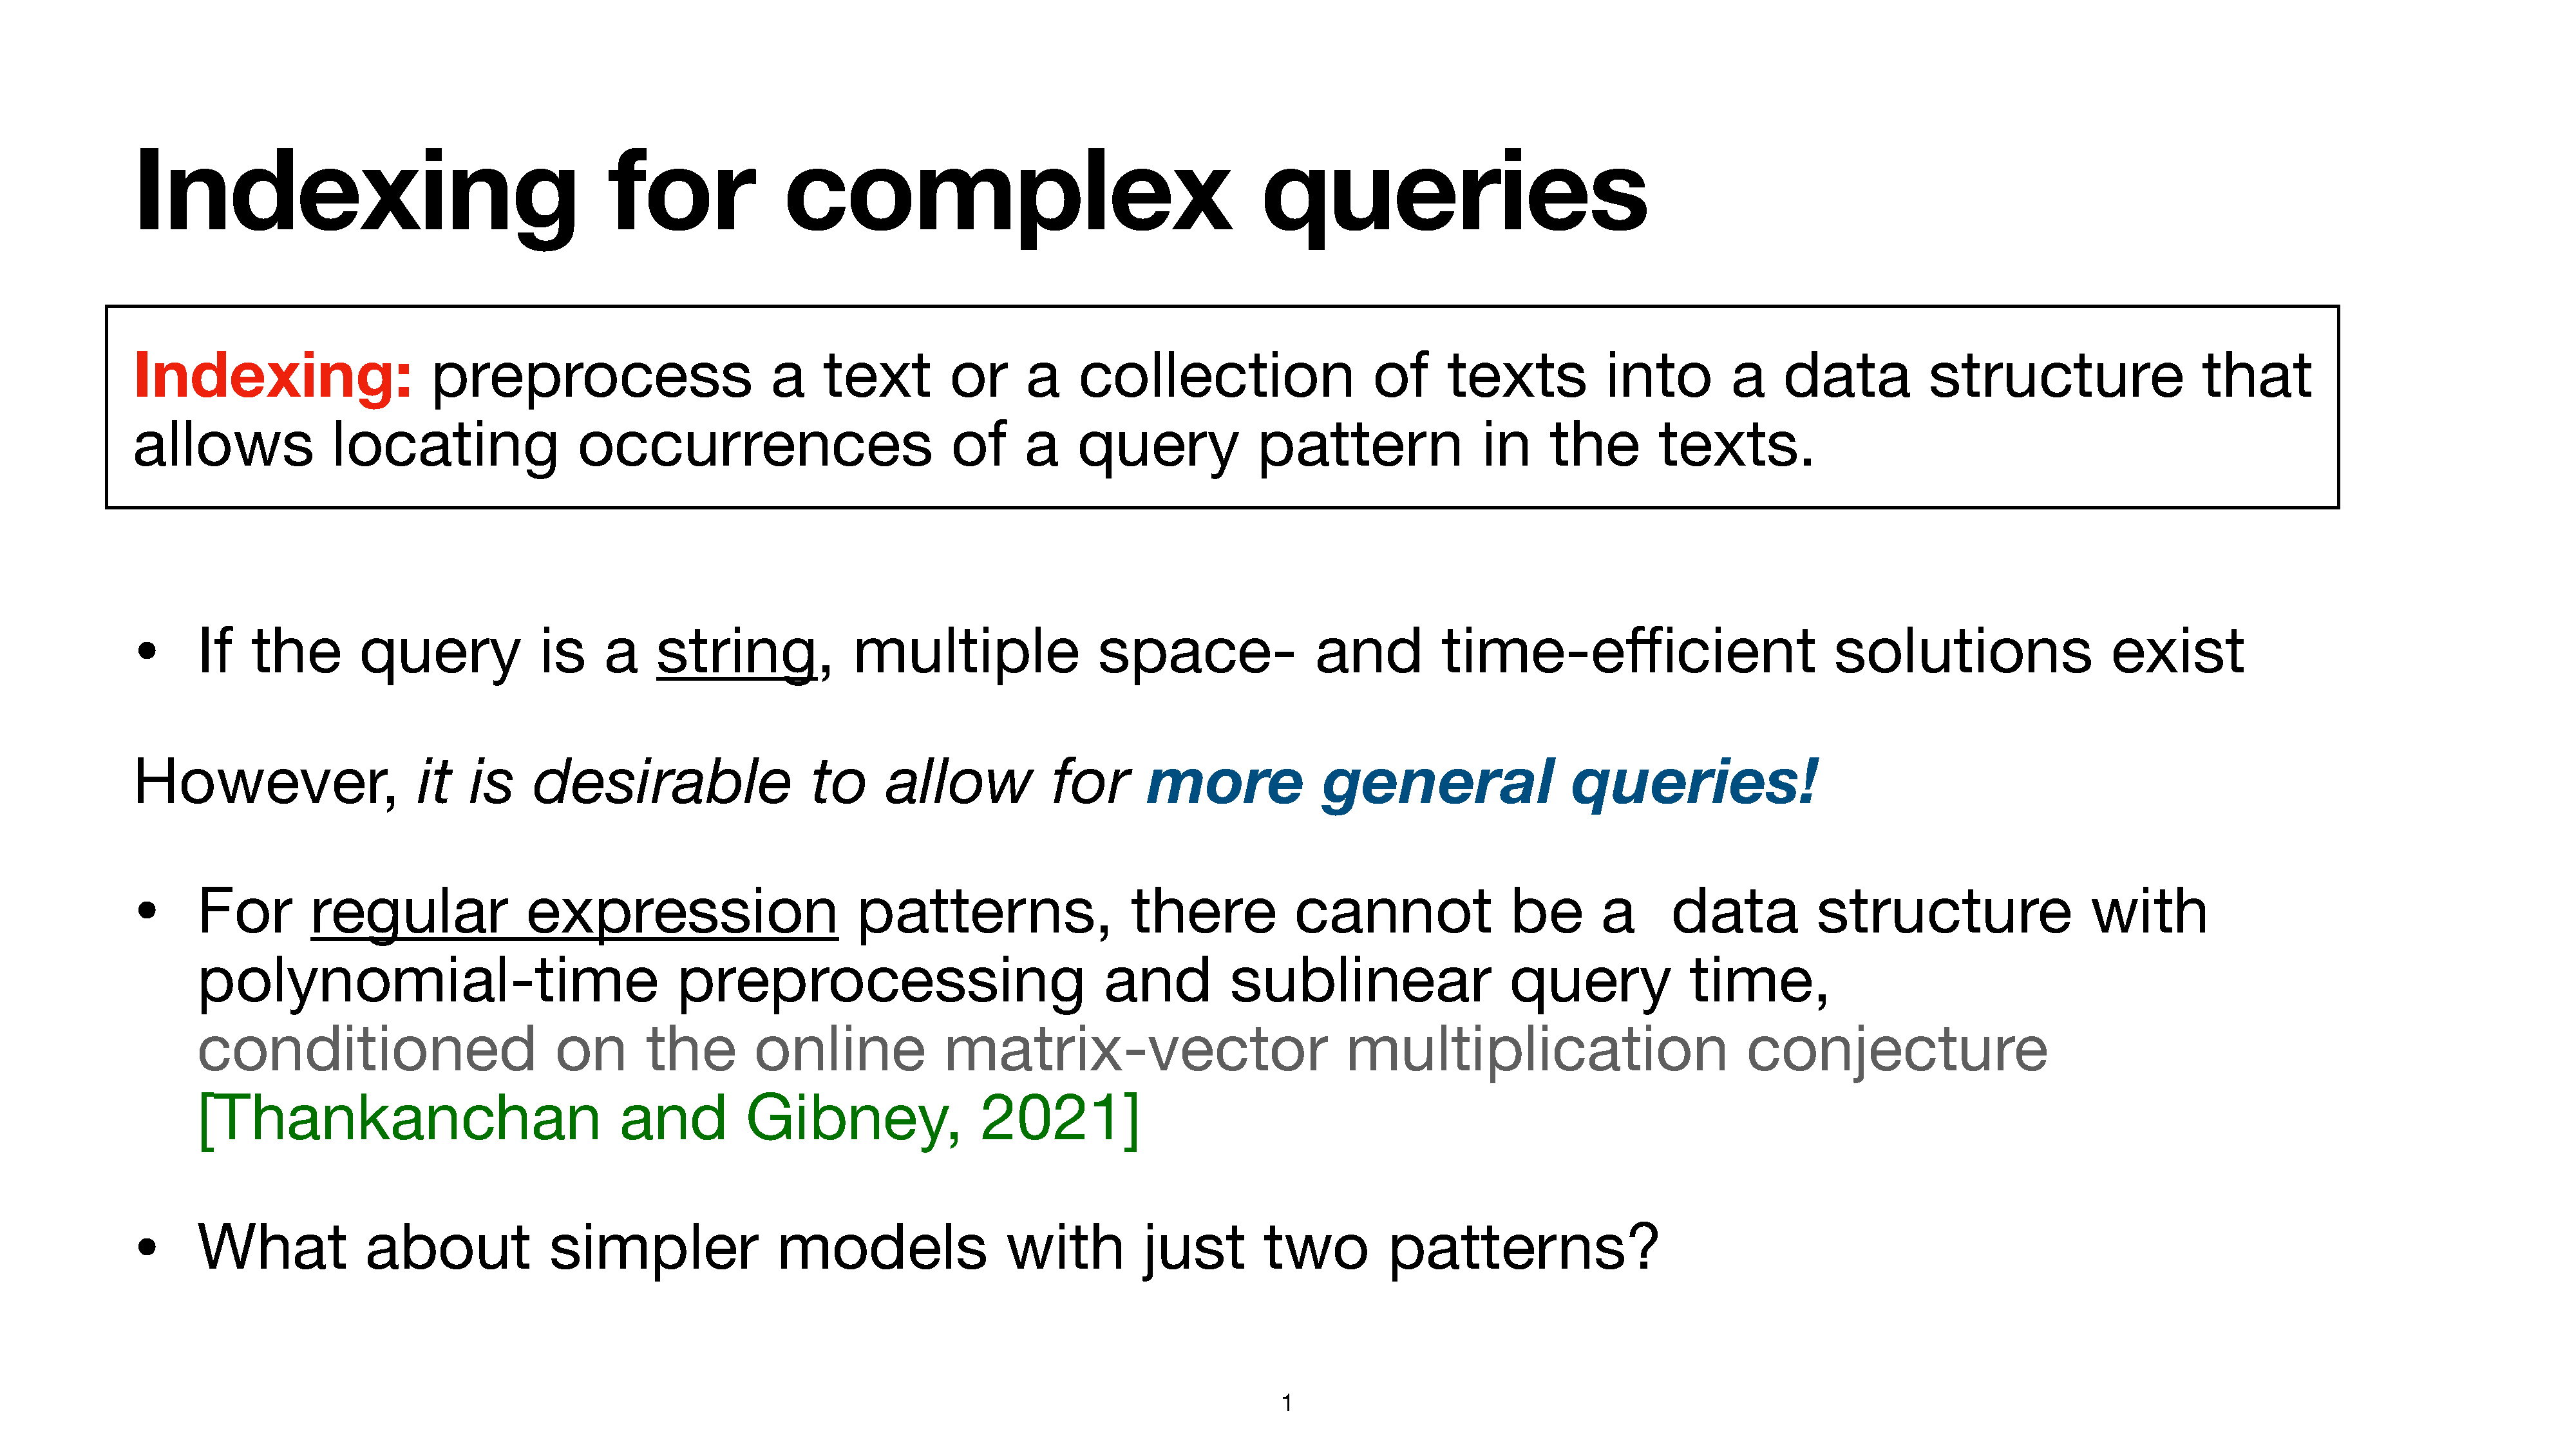
\includepdf[pages={-}]{pdf/2_index_gapped.pdf}



\newcommand{\kLCS}{\textsf{LCS with $k$ Mismatches}}
\newcommand{\kApproxLCS}{\textsf{LCS with Approximately $k$ Mismatches}}
\newcommand{\acs}{\mathrm{ACS}}
\newcommand{\lcpk}{\mathrm{LCP}_{k}}
\newcommand{\lcpe}{\mathrm{LCP}_{(1+\eps)k}}
\newcommand{\Projections}{\Pi}
\newcommand{\Hashes}{\mathcal{H}}
\newcommand{\Collisions}{C}
\newcommand{\HD}{d_H}
\newcommand{\sk}{\mathrm{sk}}
\newcommand{\norm}[1]{\ensuremath{\lVert#1\rVert}}
\newcommand{\Ham}{\mathrm{Ham}}


\subsection{LCS(ubstring) with Approximately k Mismatches}
\begin{frame}
  \centering
  \beamermathcolor{black}
  {\Large The Longest Common Substring with Approximately $k$ Mismatches}
  
  \medskip
  {\large CPM'20}
  \bigskip

  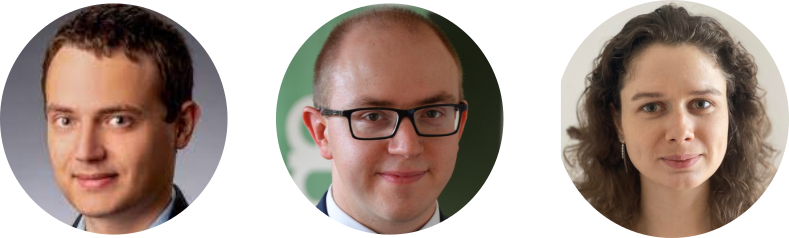
\includegraphics{pictures/mindmap/lcsk.png}

  \bigskip
  Tomasz Kociumaka, Jakub Radoszewski, Tatiana Starikovskaya
\end{frame}


\frame{
\frametitle{The Longest Common Substring with Approximately $k$ mismatches}
\begin{block}{$LCS_{\tilde{k}}$}
\textbf{Input}: Two strings $X, Y$ of length $n$, an integer $k$.\\
\textbf{Output}: A substring of $X$ of length at least $LCS_k$ that occurs in $Y$ with at most $(1+\eps) \cdot k$ mismatches.
\end{block}

\pause

\begin{block}{[Kociumaka, Radosweski, Starikovskaya'19]}
  $LCS_{\tilde{k}}$ can be solved for $\eps < 2$, in $\Oh(n^{1+1/(1+\eps)}\log^2 n)$ time and $\Oh(n^{1+1/(1+\eps)})$ space.
\end{block}

}

\frame{
\frametitle{Our contributions}
\begin{myalertblock}{Upper bounds}
 Let $\eps > 0$ be an arbitrary constant. The \kApproxLCS  problem can be solved correctly with high probability: 
\begin{enumerate}[1)]
\item in $\Oh(n^{1+ 1/(1+2\eps) + o(1)} \log^2 n)$ time and $\Oh(n^{1+ 1/(1+2\eps) + o(1)})$ space assuming a constant-size alphabet;
\item and $\Oh(n^{1+1/(1+\eps)} \log^3 n)$ time and $\Oh(n)$ space for alphabets of arbitrary size. 
\end{enumerate}
\end{myalertblock}

\begin{myalertblock}{Lower Bound}
Assuming SETH, for every constant $\delta > 0$, there exists a constant $\eps = \eps(\delta)$ such that given $X$ and $Y$ of size $n$ computing the \kApproxLCS requires $\Omega(n^{2-\delta})$ time. 
\end{myalertblock}
}


\frame{
\frametitle{The Longest Common Substring problem}

\begin{block}{LCS}
\textbf{Input}: Two strings $X, Y$ of length $n$.\\
\textbf{Output}: The longest substring that occurs both in $X$ and $Y$.
\end{block}

Issue: It is not robust.
\pause
\begin{center}
$X=a^{2m+1}$ and $Y= a^{2m}b$ $\Rightarrow$ $LCS(X,Y)=2m$\\
\pause
$X=a^{m}ba^m$ and $Y= a^{2m}b$ $\Rightarrow$ $LCS(X,Y)=m$
\end{center}
\pause
Only one character changed, and the LCS has been divided by 2.
}


\frame{
\frametitle{The Longest Common Substring with $k$ mismatches}
\begin{block}{\kLCS}
\textbf{Input}: Two strings $X, Y$ of length $n$, an integer $k$.\\
\textbf{Output}: A substring of $X$ that occurs in $Y$ with at most $k$ mismatches.
\end{block}
\pause
However...
\begin{block}{[Kociumaka, Radoszweski, Starikovskaya'19]}
 There is a $k = \Theta (\log(n))$ such that $LCS_k$ can't be computed in strongly subquadratic time, unless SETH is false.
 \end{block}

}


\frame{
\frametitle{Twenty question game with a liar}

\begin{center}
\hspace{0.1\textwidth}
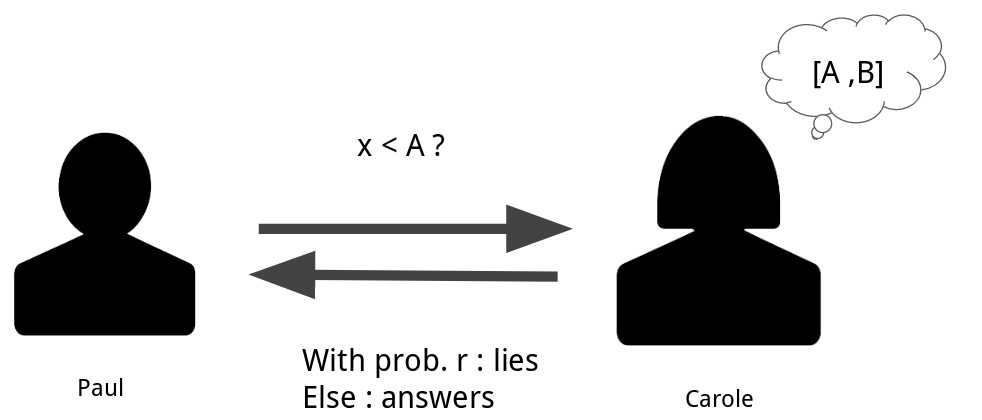
\includegraphics[width=0.8\textwidth]{figures/20q}
\end{center}

\begin{block}{[Dhagat, G{\'a}cs, Winkler '92]}
For $A = B$, Paul has a winning strategy for all $r < \frac{1}{3}$ asking $Q = \lceil \frac{8 \log N}{(1-3r)^2} \rceil =  \Theta(\log n)$ questions.
\end{block}

}

\frame{
\frametitle{Decision variant }

\btheme{Input:} integers ${k, \ell}$, a constant ${\eps > 0}$, strings ${S_1, S_2}$ of length ${n}$

\btheme{Output:} 

\begin{enumerate}
\item YES if ${\ell \le \mathrm{LCS_k}}$;
\item YES or NO if ${\mathrm{LCS_k} < \ell \le \mathrm{LCS_{(1+\eps)k}}}$; 
\item NO if ${\mathrm{LCS_{(1+\eps)k}} < \ell}$.
\end{enumerate}

The answer must be correct with probability at least $3/4$.

\pause
\par\noindent\ntheme{\rule{\textwidth}{1pt}}

\ntheme{Longest Common Substring with approx. $k$ mismatches:}

\medskip
\begin{itemize}
\item $A = \mathrm{LCS_k}$ and $B = \mathrm{LCS_{(1+\eps)k}}$.\\
\item An algorithm for the decision variant plays the role of Carole. \\
\item With ${\lceil \frac{8 \log n}{(1-3r)^2} \rceil}$ questions, Paul will find $x \in [\mathrm{LCS_k}, \mathrm{LCS_{(1+\eps)k}}]$ for some $1/4 < r < 1/3$.
\end{itemize}

}


\frame{
\frametitle{Locality-Sensitive Hashing}
Nearest Neighbour search, data clustering...\\
In string processing: Andoni and Indyk for a space-efficient randomized index for approximate pattern matching.
\pause
\begin{enumerate}
\item Projections:
\vspace{-0.5cm}
$$h(S)=S[a_{p_1}] S[a_{p_2}] \cdots S[a_{p_m}]$$
And Collisions-Sets (Karp-Rabin fingerprints).
$$\Collisions^{\Hashes}_{\ell} = \{(S_1,S_2, h) :\varphi(h(S_1 0^{n-\ell})) = \varphi(h(S_2 0^{n-\ell})) \}$$
\pause
\item Dimension reduction.
\vspace{0.1cm}
With probability at least $1- n^{-\beta}$, for all $u,v \in P$:\\
\begin{enumerate}[1)]
\item if $\norm{\sk_\alpha(u)-\sk_\alpha(v)}^2 \le (1+\alpha) \cdot k$, then $\HD(u,v) \le (1+\alpha) \cdot k$;
\item if $\norm{\sk_\alpha(u)-\sk_\alpha(v)}^2 > (1+\alpha) \cdot k$, then $\HD(u,v) \ge k$.
\end{enumerate}
\end{enumerate}
}



\frame{
\frametitle{Algorithm}

\begin{algorithm}[H]
\small
%\caption{LCS with approx. $k$ mismatches, decision variant}
\begin{algorithmic}[1]
\State Choose a set $\ntheme{\Hashes}$ of ${\Theta(n^{1/(1+\eps)})}$ functions from ${\Projections^m}$ u.a.r.
\State $\ntheme{\Collisions^{\Hashes}_{l} :=}$ set of all collisions of $l$-length substrings of $\ntheme{S_1, S_2}$ under the hash functions in $\ntheme{\Hashes}$
\State Draw a collision $\ntheme{(X, Y) \in \Collisions^{\Hashes}_{\ell}}$ uniformly at random 
\If {$\ntheme{\Ham (X, Y) \le (1+\eps) \cdot k}$}
	\Return YES
\EndIf
\State Choose a subset $\ntheme{\Collisions' \subseteq \Collisions^{\Hashes}_{l}}$ of size $\ntheme{\min\{\Collisions^{\Hashes}_{\ell}, 4nL\}}$
\For {$\ntheme{(X, Y) \in \Collisions'}$} 
	\If {$\ntheme{\Ham(S_1, S_2) \le k}$} 
		\Return YES
	\EndIf
\EndFor
\State \Return NO
\end{algorithmic}
\end{algorithm}

\pause
\ntheme{Running time $\Oh(n^{1+1/(1+\eps)} \log n)$:}
\begin{enumerate}
\item Compute the hash values and $\Collisions'$: $\Oh(n^{1+1/(1+\eps)} \log n)$ time (FFT)

\item Pick a random collision: $\Oh(n^{1+1/(1+\eps)})$ time (reservoir sampling)

\item Test in line 5: $\Oh(n^{1+1/(1+\eps)} \log^2 n)$ time (dimension reduction)

\item Test in line 7: $\Oh(n)$ time (character-by-character)
\end{enumerate}
}

\frame{
\frametitle{Experiments}

None of the previous solutions have been implemented. 

The only algorithm that seemed to be practical enough is the dynamic programming one \ntheme{[Flouri et al.'15]}

\pause
\bigskip

We compared our algorithm with the dynamic programming one
\begin{itemize}
 \item On random strings;
 \item On strings extracted from E. coli.
\end{itemize}

\medskip

Lengths from $5000$ to $60000$, $k = 10, 25, 50$
}

\frame{
\frametitle{Adjustments to the theory}
Implemented in C++ available on github.
\begin{enumerate}

\item Sketching for the Hamming distance via dimension reduction: replaced by a naive comparison character by character, Bit parallelism.
\pause

\item Computation of the collisions: A naive implementation, FFT and NTT.
\pause

\item The twenty question game: the twenty question game, binary search.
\pause

\item The number of hash functions $L$: $L = n^{1/(1+\eps)}$, $L = n^{1/(1+\eps)}/\log(n)$.

\end{enumerate}

}

\frame{
\frametitle{Running time}


\begin{figure}[ht!]
\centering
    \begin{subfigure}{.5\textwidth}
        \centering
        \captionsetup{justification=centering}
        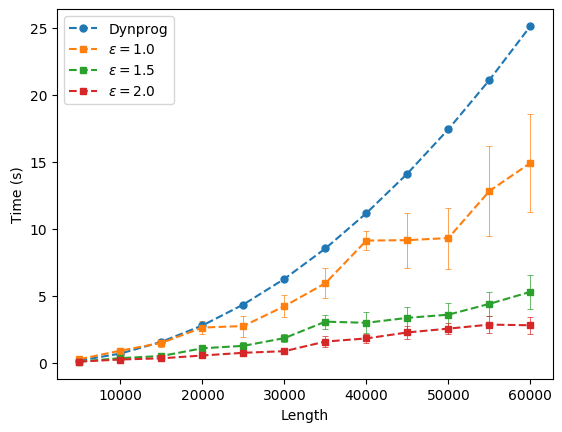
\includegraphics[scale=0.4]{figures/random_25.png}
        \caption{Random, $k = 25$}
    \end{subfigure}%
    \begin{subfigure}{0.5\textwidth}
        \centering
        \captionsetup{justification=centering}
        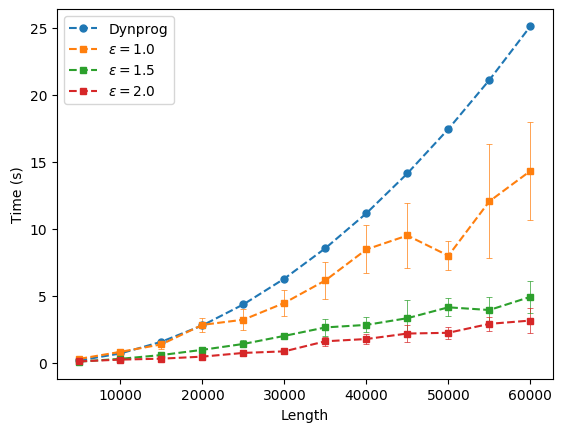
\includegraphics[scale=0.4]{figures/e_coli_25.png}
        \caption{E. coli, $k = 25$}
    \end{subfigure}     

\end{figure}


\bigskip

\begin{itemize}
\item For each length, we performed $10$ independent experiments
\item Big standard deviation for $\eps = 1$, negligible for $\eps = 1.5$ and $\eps = 2.0$
\item Gain up to a factor of 10 on strings of length $60000$
\end{itemize}
}



\frame{
\frametitle{Distortion and accuracy}

\begin{columns}
\column{0.5\textwidth}    
{\small
We estimate distortion by computing two values:

$r_{\min}(\eps, k) = \min_{S_1,S_2}(\mathrm{LCS_{\tilde{k}}}(S_1,S_2)/\mathrm{LCS_k}(S_1,S_2))$\\
$r_{\max}(\eps, k) = \max_{S_1,S_2}(\mathrm{LCS_{\tilde{k}}}(S_1,S_2)/\mathrm{LCS_k}(S_1,S_2))$

Furthermore, we can only err by returning a string shorter than $\mathrm{LCS_k}$.
}

\column{0.6\textwidth}

\newcolumntype{?}{!{\vrule width 1pt}}
\newcommand{\err}{\textcolor{red}{\mathrm{err}}}
\begin{center}
\begin{table}
\begin{tabular}{|l?l|l|l|l|l|l|}
\hline
 & \multicolumn{6}{c|}{\ntheme{Random}}\\ 
\hline
 & \multicolumn{2}{c|}{$\eps = 1.0$} & \multicolumn{2}{|c|}{$\eps = 1.5$} & \multicolumn{2}{|c|}{$\eps = 2.0$}\\ 
\hline

\multirow{ 2}{*}{$k = 10$} & 0.92 & 1.50 & 1.00 & 1.53 & 1.13 & 1.87\\ 
\cline{2-7}
& \multicolumn{2}{c|}{$\err = 7\%$}  & \multicolumn{2}{c|}{$\err = 0\%$}   & \multicolumn{2}{c|}{$\err = 0\%$}\\ 
\hline
\multirow{ 2}{*}{$k = 25$}  & 1.10 & 1.48 & 1.30 & 1.70 & 1.55 & 2.11\\ 
\cline{2-7}
& \multicolumn{2}{c|}{$\err = 0\%$}  & \multicolumn{2}{c|}{$\err = 0\%$}   & \multicolumn{2}{c|}{$\err = 0\%$}\\ 
\hline
\hline

& \multicolumn{6}{c|}{\ntheme{E. coli}} \\ 
\hline
& \multicolumn{2}{|c|}{$\eps = 1.0$} & \multicolumn{2}{c|}{$\eps = 1.5$} & \multicolumn{2}{c|}{$\eps = 2.0$} \\ 
\hline

\multirow{ 2}{*}{$k = 10$} & 0.86 & 1.41 & 0.91 & 1.47 & 0.95 & 1.71\\ 
\cline{2-7}
& \multicolumn{2}{|c|}{$\err = 34\%$}   & \multicolumn{2}{c|}{$\err = 13\%$}  & \multicolumn{2}{c|}{$\err = 8\%$}\\ 
\hline
\multirow{ 2}{*}{$k = 25$}  & 0.94  & 1.45 & 0.96 & 1.75 & 0.98 & 1.96\\ 
\cline{2-7}
& \multicolumn{2}{c|}{$\err = 7\%$}   & \multicolumn{2}{c|}{$\err = 5\%$}  & \multicolumn{2}{c|}{$\err = 2\%$}\\ 
\hline

\end{tabular} 
\label{tb:eps}
\end{table}
\end{center}


\end{columns}

}

\section{Bonus DTW}

\begin{frame}
  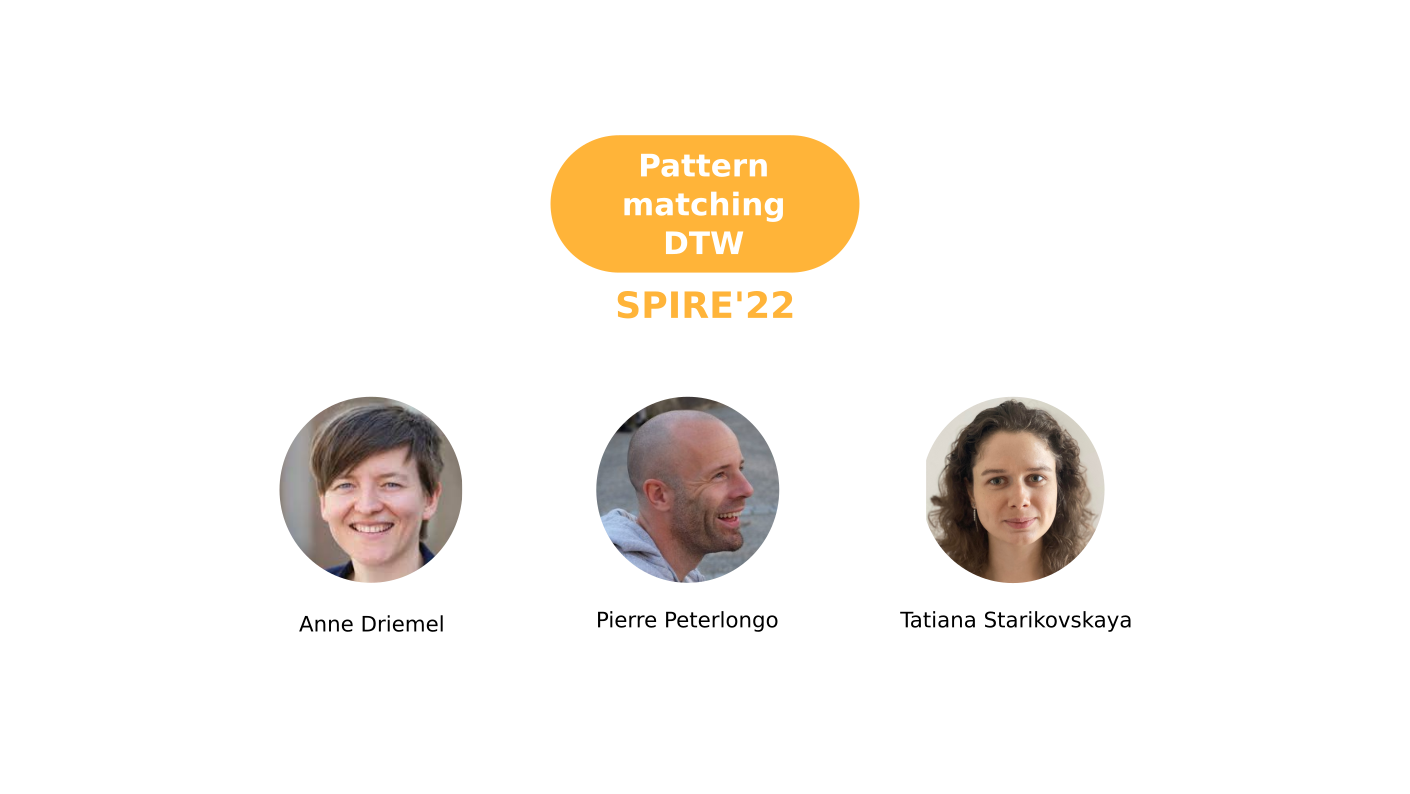
\includegraphics[width=\textwidth]{pictures/mindmap/dtw.png}
\end{frame}

\begin{frame}{Formal definition of $\dtw(X,Y)$ and dynamic programming}

  \begin{columns}
  \column{0.45\textwidth}
  \newcommand{\dtwgrid}[2]{% height width 
\foreach \i in {0,...,#1} {
	\foreach \j in {0,...,#2} {
		\filldraw[black] (\i , \j) circle (2pt);
		\ifthenelse{ \not \equal{#2}{\j}}{ 
			\draw[->] ($(\i , \j+0.9)$) -- ($(\i , \j+0.1)$);
		}{}
		\ifthenelse{ \not \equal{#1}{\i}}{
  			\draw[->] ($(\i +0.1 , \j)$) -- ($(\i +0.9 , \j)$);
		}{}
		\ifthenelse{\not\equal{#1}{\i} \and \not \equal{#2}{\j}}{%
  			\draw[->] ($(\i +0.1 , \j + 0.9)$) -- ($(\i +0.9, \j + 0.1)$);
  		}{}
	}
}
}

\newcommand{\dtwarrow}[2]{%
\draw[->,line width=0.3mm,red] #1 -- #2;
}

  \begin{figure}
      \beamermathcolor{black}
      \centering
      \begin{tikzpicture}[scale=0.8, every node/.style={scale=1.2}]
      \dtwgrid{5}{2}
  
      \foreach \i in {1,...,6} {
          \node at ($(\i-1, 2.8)$) {\tiny{$X[\i]$}};
      }
      \foreach \j in {1,...,3} {
          \node at ($(-1.2, 3 -\j )$) {\tiny{$Y[\j]$}};
      }
  
      \foreach \x[count=\i] in {C,A,A,A,G,G} {
          \node at ($(\i-1 , 2.3)$) {\textcolor{black}{\tiny{\x}}};
      }
      \foreach \y[count=\j] in {A,T,G} {
          \node at ($(-0.5, 3 -\j )$) {\textcolor{black}{\tiny{\y}}};
      }
  
  
      \only<2->{
          \dtwarrow{(0.1,2)}{(0.9,2)}
          \dtwarrow{(3.1,1.9)}{(3.9,1.1)}
          \dtwarrow{(1.1,2)}{(1.9,2)}
          \dtwarrow{(2.1,2)}{(2.9,2)}
          \dtwarrow{(4,0.9)}{(4,0.1)}
          \dtwarrow{(4.1,0)}{(4.9,0)}
          \node at (5,-0.3) {\bred{$\pi$}};
      }
  
      \end{tikzpicture}
  \end{figure}
  \column{0.45\textwidth}
  \centering
  \only<3>{
  $\text{cost}(\pi) = \sum_{(i,\ j)\in \pi} d(X[i],Y[j])$\\
  \vspace{0.5cm}
  $\dtw(X,Y) = \min_{\pi} \text{cost}(\pi)$\\
  \vspace{0.5cm}
  {\small s.t. $\pi$ goes from top left to bottom right.}}
  \end{columns}
  \pause %grid definition 
  \pause %draw the path
  \pause
  
  \bigskip
  
  
  \only<4|handout:0>{
  \begin{exampleblock}{Path correspondance to alignment}
  \center
  \begin{figure}
  %\missingfigure{Under construction...}
  \centering
  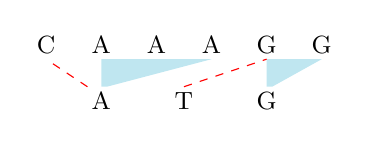
\begin{tikzpicture}[scale=0.7, every node/.style={scale=1}]
  \foreach \x[count=\i] in {C,A,A,A,G,G} {
      \node at ($(\i, 1)$) {\small{\x}};
  }
  \foreach \y[count=\j] in {A,T,G} {
      \node at ($(0.5+\j*1.5, 0)$) {\small{\y}};
  }
  % align A
  \fill[myblue!25] (2, 0.25) -- (2,0.75) -- (4,0.75) -- (2.1,0.25) -- cycle;
  % align G
  \fill[myblue!25] (5, 0.25) -- (5,0.75) -- (6,0.75) -- (5.1,0.25) -- cycle;
  %draw misalignment
  \draw[dashed,red] (1.75, 0.25) -- (1,0.75);
  \draw[dashed,red] (3.5, 0.25) -- (5,0.75);
  \end{tikzpicture}
  \end{figure}
  \vfill
  $\dtw($CAAAG$,$ATG$)=2$
  \end{exampleblock}}
  
  \only<5->{
  
  \btheme{Dynamic Programming solution}\\
  \smallskip
  $D$ a matrix of size $(M+1)(N+1)$ such that $D[i,j]=\dtw(X[1..i],Y[1..j])$\pause
  \bigskip
  
  \btheme{Initialization}~~~$D[0,0]= 0$ and for all $(i,j)$, $D[0,j]=D[i,0]=+\infty$.\\
  \pause
  \bigskip
  \btheme{Recurrence} ~~~ 
      $D[i,j] = \min\{$\beamermathcolor{black}
          $\underbrace{\mathcolor{black!30!blue}{D[i-1,j-1]}}_\text{top-left},
          \underbrace{\mathcolor{black!30!blue}{D[i-1,j]}}_\text{top},
          \underbrace{\mathcolor{black!30!blue}{D[i,j-1]}}_\text{left}$
      $\mathcolor{black!30!blue}{\}+ d(X[i], Y[j])}$.
  }
  
  \end{frame}
  

\begin{frame}{}

  \textbf{Our contributions:}\\
  For $T$ and $P$ two strings, $|T|=N$ and  $|P|=M$, $|\RLE(T)|=n$ and  $|\RLE(P)|=m$.
  Pattern matching under DTW distance:
  \begin{itemize}
  \item $\Oh(Nm+nM)$-time general algorithm which can for an integer distance, compute all values bellow $k$ in $\Oh(nmk)$-time. \pause
  \item Toy implementation available on github.\pause
  \item An $\Oh(L^{\eps})$-approximation, for any $0 < \eps < 1$, in  $\Oh(L^{1-\eps} \cdot mn \log^3 L)$-time with $L=\max(N,M)$.\pause
  \item (A $\Oh(n+m)$-time algorithm for $k=1$.)\pause
  \end{itemize}
  
  
  \textbf{Open questions:}
  \begin{itemize}
  \item Is a $\Oh(k(n+m))$-time algorithm possible? \pause
  \item Can those improvements benefit applications ?\pause
  \end{itemize}
  \end{frame}


\begin{frame}{Experiments: visualization on simulated data}
  Problem: How to design a protocol that isn't biased towards ED ?\\
  Model to illustrate the impact of homopolymers on ED.
  \begin{center}
    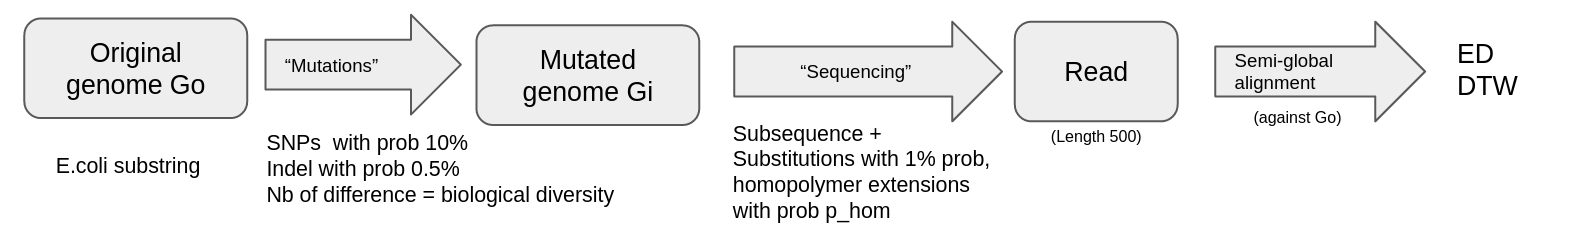
\includegraphics[scale=0.2]{figures/pipeline.png}
  \end{center}
  \vspace{-0.5cm}
  \begin{columns}
    \column{0.3\textwidth}
    
    We compare the values of the two distances as the probability of extending homopolymers increases.
    
    \column{0.5\textwidth}
    \begin{center}
      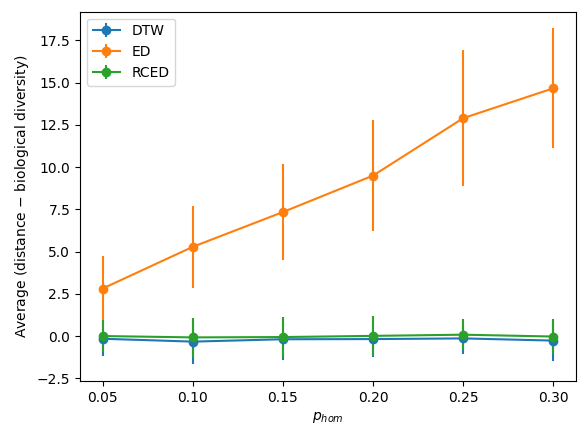
\includegraphics[scale=0.4]{figures/ecoli_10kb_N_100_fixed_ID_0.0005.png}
    \end{center}
  \end{columns}
\end{frame}


\begin{frame}{Comparison to the edit distance}
  \beamermathcolor{black}
  \[
  D[i,j] = {\min\{
  \underbrace{D[i-1,j-1]}_\text{top-left},
  \underbrace{D[i-1,j]}_\text{top},
  \underbrace{D[i,j-1]}_\text{left}
  \} \mathcolor{red}{+ d(X[i], Y[j])}
  }
      \]
  
  \[
  ED[i,j] = {\min\{
  \underbrace{ED[i-1,j-1]}_\text{top-left} \mathcolor{red}{+ d(X[i], Y[j])},
  \underbrace{ED[i-1,j]}_\text{top} \mathcolor{red}{+1},
  \underbrace{ED[i,j-1]}_\text{left} \mathcolor{red}{+1}
  \}
  }
      \]
  
  \pause
  
  \only<2-3|handout:0>{
  \begin{exampleblock}{DTW vs ED}
  $\ed(AAAA\mathcolor{myblue}{T}G,AA\mathcolor{myblue}{T}C)=3$ whereas $\dtw(AAAA\mathcolor{myblue}{T}G,AA\mathcolor{myblue}{T}C)=1$.\\
  $\dtw(AAAA\mathcolor{myblue}{T}G,AA\mathcolor{myblue}{T}CCC)=3$
  \end{exampleblock} 
  
  \only<3>{$\Rightarrow$ Compresses runs of matching letters!}
  }

  \only<4>{
    \begin{center}
      
\begin{center}
\footnotesize
\resizebox{0.8\textwidth}{!}{
\begin{tabular}{|cc||cc|cccc|c|cc|c|cccc|cc|c|c|c|c|c|}
\hline
 &   & G & G & T & T & T & T & C & T & T & A & T & T & T & T & G & G & T & G & A & T & A \\
 & 0 & 0 & 0 & 0 & \textcolor{red}{0} & 0 & 0 & 0 & 0 & 0 & 0 & 0 & 0 & 0 & 0 & 0 & 0 & 0 & 0 & 0 & 0 & 0 \\
\hline
A  & $\infty$  & 1 & 1 & 1 & 1 & \textcolor{red}{1} & 1 & 1 & 1 & 1 &{ 0 } & 1 & 1 & 1 & 1 & 1 & 1 & 1 & 1 &{ 0 } & 1 &{ 0 }\\
A  & $\infty$  & 2 & 2 & 2 & 2 & 2 & \textcolor{red}{2} & 2 & 2 & 2 &{ 0 } & 1 & 2 & 2 & 2 & 2 & 2 & 2 & 2 &{ 0 } & 1 &{ 0 }\\
\hline
T  & $\infty$  & 3 & 3 &{ 2 } &{ 2 } &{ 2 } &{ 2 } & \textcolor{red}{3} &{{ 2 }} &{{ 2 }} & 1 &{ 0 } &{ 0 } &{ 0 } &{ 0 } & 1 & 2 &{ 2 } & 3 & 1 &{ 0 } & 1\\
T  & $\infty$  & 4 & 4 &{ 2 } &{ 2 } &{ 2 } &{ 2 } & 3 & \textcolor{red}{{ 2 }} &{{ 2 }} & 2 &{ 0 } &{ 0 } &{ 0 } &{ 0 } & 1 & 2 &{ 2 } & 3 & 2 &{ 0 } & 1\\
\hline
A  & $\infty$  & 5 & 5 & 3 & 3 & 3 & 3 & 3 & 3 & \textcolor{red}{3} &{{ 2 }} & 1 & 1 & 1 & 1 & 1 & 2 & 3 & 3 &{ 2 } & 1 &{ 0 }\\
\hline
T  & $\infty$  & 6 & 6 &{ 3 } &{ 3 } &{ 3 } &{ 3 } & 4 &{ 3 } &{ 3 } & \textcolor{red}{3} &{{ 1 }} &{{ 1 }} &{{ 1 }} &{{ 1 }} & 2 & 2 &{ 2 } & 3 & 3 &{ 1 } & 1\\
\hline

\end{tabular} }
\end{center}



\pause
    \end{center}
    \small{Unlike for the edit distance, \textcolor{red}{diagonals can be non-monotone}.}
  }
      
  \end{frame}

\section{XBWT indexing of aligned readsets}
\begin{frame}
  \centering
  {\Large XBWT indexing of aligned readsets}
    
  \medskip
  {\large WABI'21}
  \bigskip

  
\includegraphics{pictures/mindmap/xbwt.png}

  \bigskip
  Travis Gagie, Giovanni Manzini
\end{frame}

%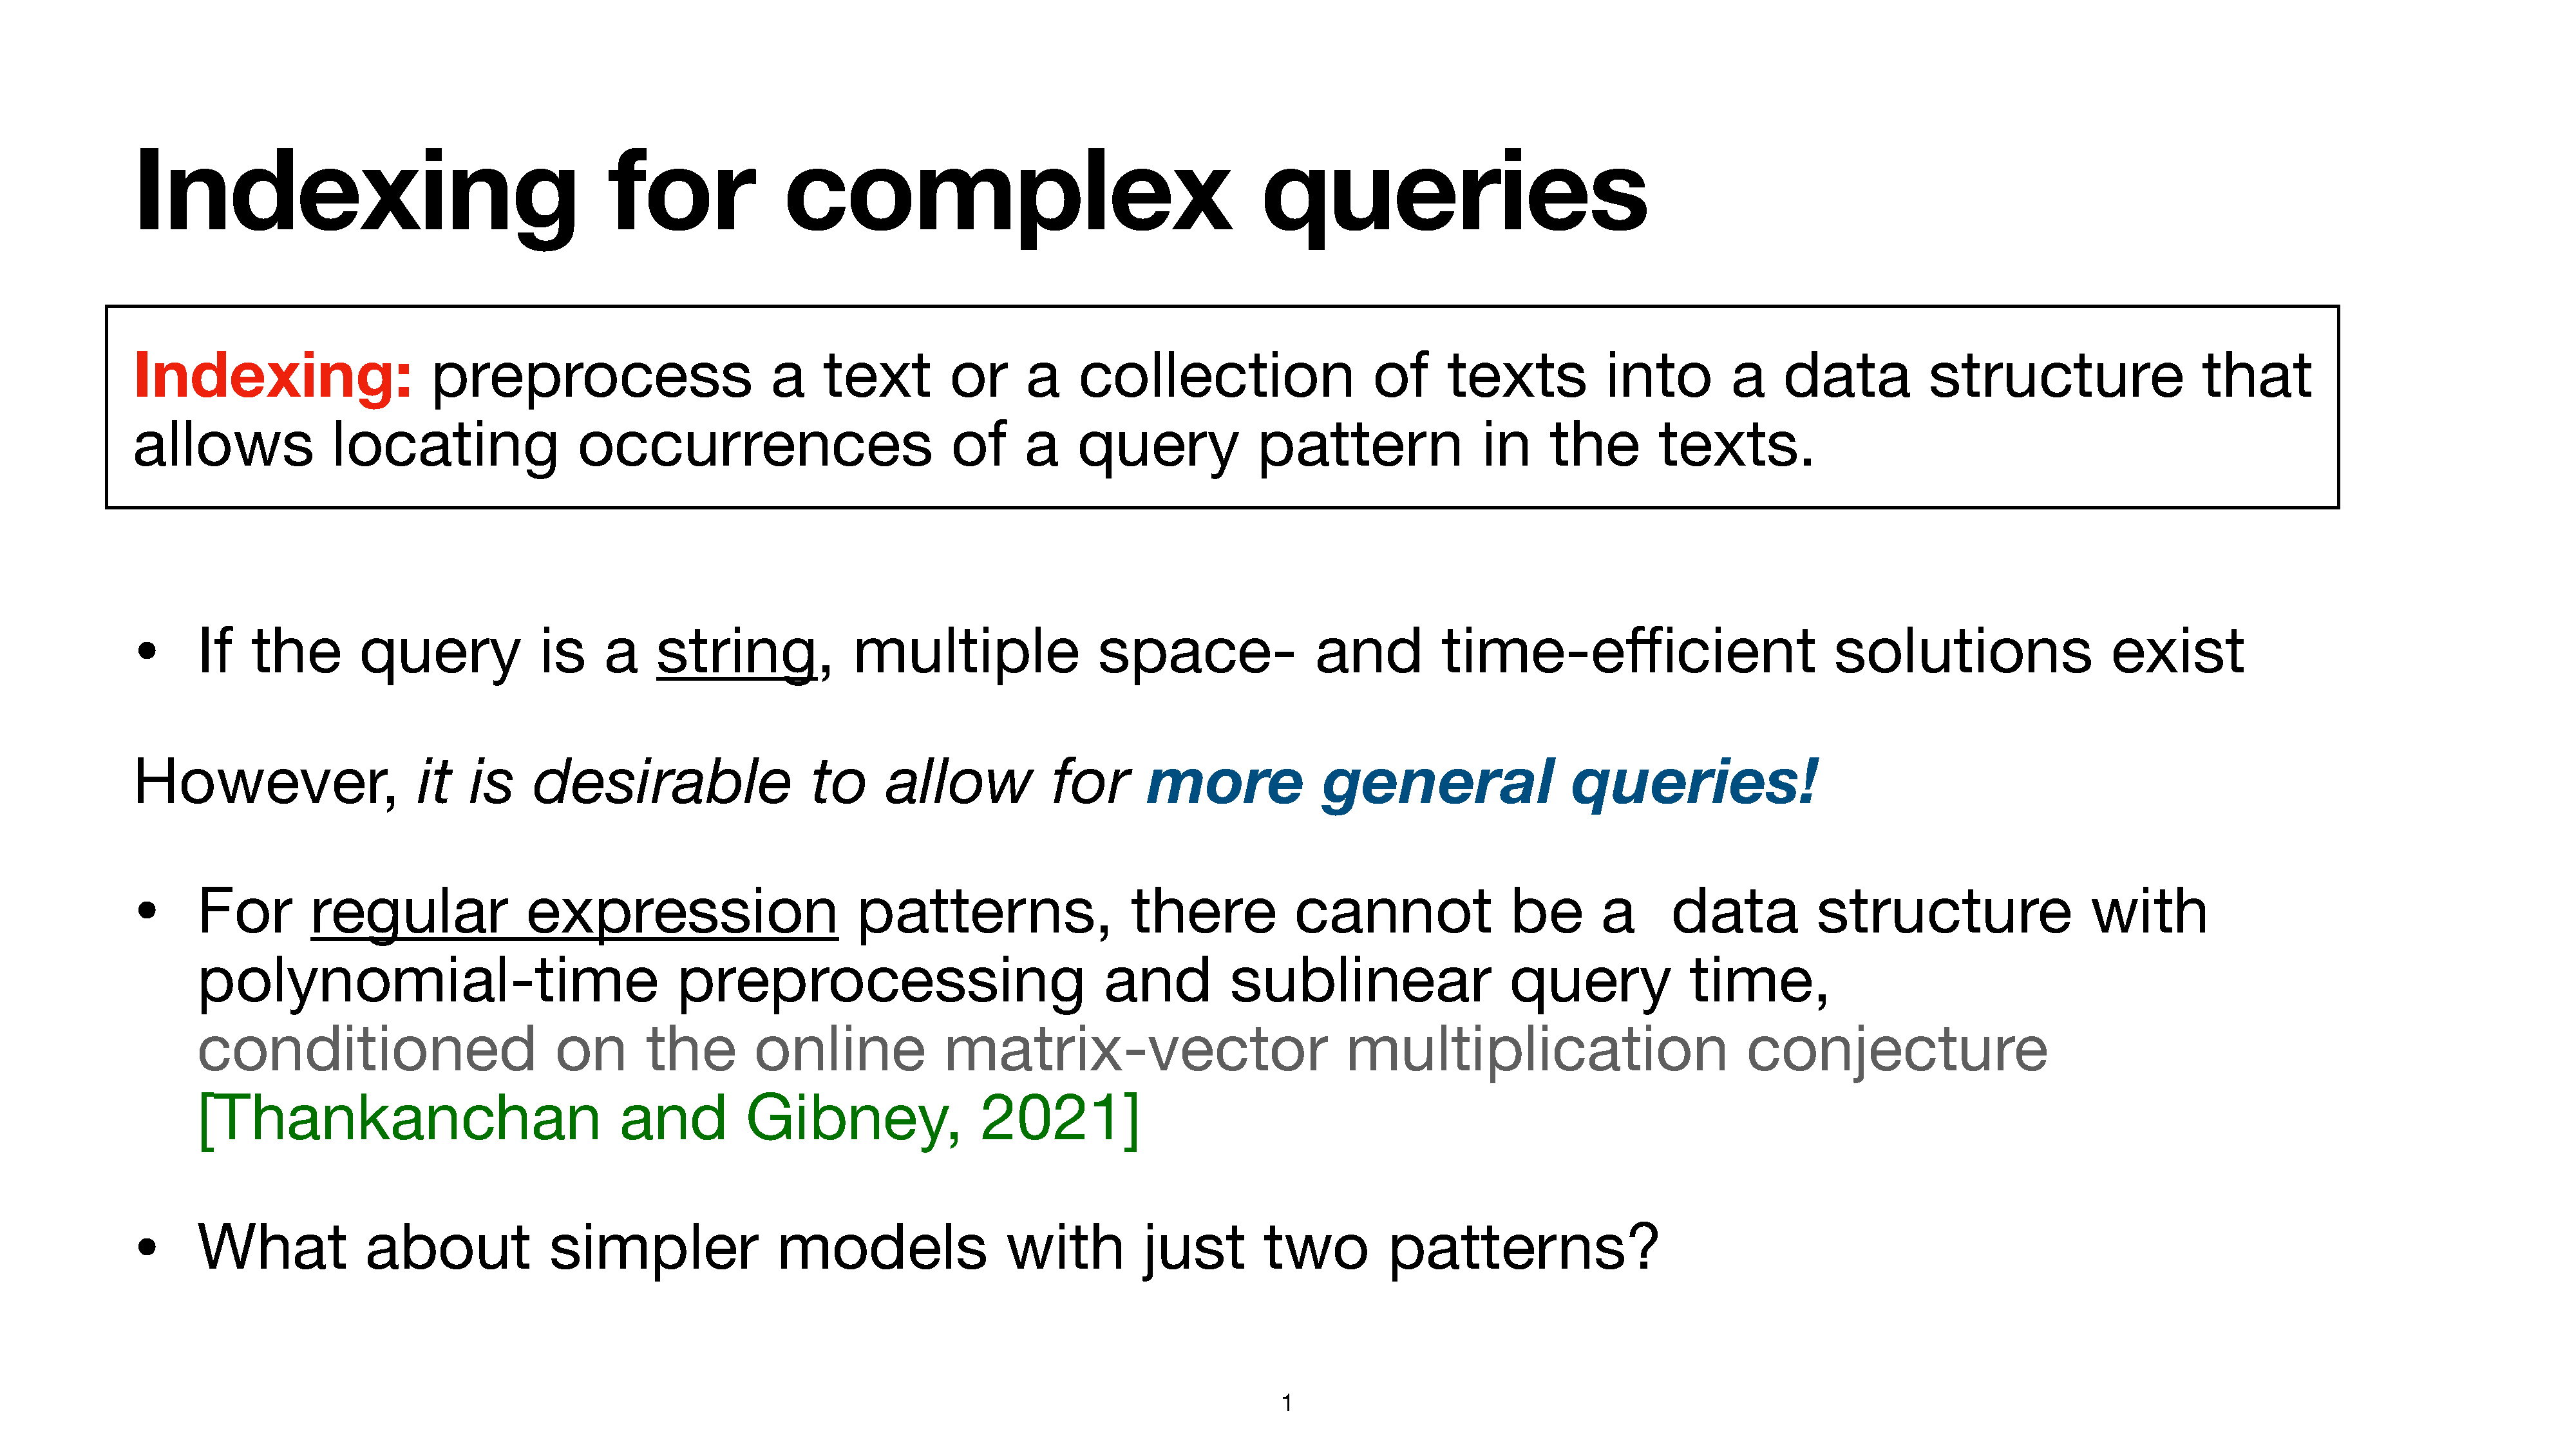
\includepdf[pages={-}]{pdf/2_index_gapped.pdf}

\backupend



\begin{frame}
  \tableofcontents
\end{frame}
\backupend

\end{document}